\documentclass[1p]{elsarticle_modified}
%\bibliographystyle{elsarticle-num}

%\usepackage[colorlinks]{hyperref}
%\usepackage{abbrmath_seonhwa} %\Abb, \Ascr, \Acal ,\Abf, \Afrak
\usepackage{amsfonts}
\usepackage{amssymb}
\usepackage{amsmath}
\usepackage{amsthm}
\usepackage{scalefnt}
\usepackage{amsbsy}
\usepackage{kotex}
\usepackage{caption}
\usepackage{subfig}
\usepackage{color}
\usepackage{graphicx}
\usepackage{xcolor} %% white, black, red, green, blue, cyan, magenta, yellow
\usepackage{float}
\usepackage{setspace}
\usepackage{hyperref}

\usepackage{tikz}
\usetikzlibrary{arrows}

\usepackage{multirow}
\usepackage{array} % fixed length table
\usepackage{hhline}

%%%%%%%%%%%%%%%%%%%%%
\makeatletter
\renewcommand*\env@matrix[1][\arraystretch]{%
	\edef\arraystretch{#1}%
	\hskip -\arraycolsep
	\let\@ifnextchar\new@ifnextchar
	\array{*\c@MaxMatrixCols c}}
\makeatother %https://tex.stackexchange.com/questions/14071/how-can-i-increase-the-line-spacing-in-a-matrix
%%%%%%%%%%%%%%%

\usepackage[normalem]{ulem}

\newcommand{\msout}[1]{\ifmmode\text{\sout{\ensuremath{#1}}}\else\sout{#1}\fi}
%SOURCE: \msout is \stkout macro in https://tex.stackexchange.com/questions/20609/strikeout-in-math-mode

\newcommand{\cancel}[1]{
	\ifmmode
	{\color{red}\msout{#1}}
	\else
	{\color{red}\sout{#1}}
	\fi
}

\newcommand{\add}[1]{
	{\color{blue}\uwave{#1}}
}

\newcommand{\replace}[2]{
	\ifmmode
	{\color{red}\msout{#1}}{\color{blue}\uwave{#2}}
	\else
	{\color{red}\sout{#1}}{\color{blue}\uwave{#2}}
	\fi
}

\newcommand{\Sol}{\mathcal{S}} %segment
\newcommand{\D}{D} %diagram
\newcommand{\A}{\mathcal{A}} %arc


%%%%%%%%%%%%%%%%%%%%%%%%%%%%%5 test

\def\sl{\operatorname{\textup{SL}}(2,\Cbb)}
\def\psl{\operatorname{\textup{PSL}}(2,\Cbb)}
\def\quan{\mkern 1mu \triangleright \mkern 1mu}

\theoremstyle{definition}
\newtheorem{thm}{Theorem}[section]
\newtheorem{prop}[thm]{Proposition}
\newtheorem{lem}[thm]{Lemma}
\newtheorem{ques}[thm]{Question}
\newtheorem{cor}[thm]{Corollary}
\newtheorem{defn}[thm]{Definition}
\newtheorem{exam}[thm]{Example}
\newtheorem{rmk}[thm]{Remark}
\newtheorem{alg}[thm]{Algorithm}

\newcommand{\I}{\sqrt{-1}}
\begin{document}

%\begin{frontmatter}
%
%\title{Boundary parabolic representations of knots up to 8 crossings}
%
%%% Group authors per affiliation:
%\author{Yunhi Cho} 
%\address{Department of Mathematics, University of Seoul, Seoul, Korea}
%\ead{yhcho@uos.ac.kr}
%
%
%\author{Seonhwa Kim} %\fnref{s_kim}}
%\address{Center for Geometry and Physics, Institute for Basic Science, Pohang, 37673, Korea}
%\ead{ryeona17@ibs.re.kr}
%
%\author{Hyuk Kim}
%\address{Department of Mathematical Sciences, Seoul National University, Seoul 08826, Korea}
%\ead{hyukkim@snu.ac.kr}
%
%\author{Seokbeom Yoon}
%\address{Department of Mathematical Sciences, Seoul National University, Seoul, 08826,  Korea}
%\ead{sbyoon15@snu.ac.kr}
%
%\begin{abstract}
%We find all boundary parabolic representation of knots up to 8 crossings.
%
%\end{abstract}
%\begin{keyword}
%    \MSC[2010] 57M25 
%\end{keyword}
%
%\end{frontmatter}

%\linenumbers
%\tableofcontents
%
\newcommand\colored[1]{\textcolor{white}{\rule[-0.35ex]{0.8em}{1.4ex}}\kern-0.8em\color{red} #1}%
%\newcommand\colored[1]{\textcolor{white}{ #1}\kern-2.17ex	\textcolor{white}{ #1}\kern-1.81ex	\textcolor{white}{ #1}\kern-2.15ex\color{red}#1	}

{\Large $\underline{12a_{0703}~(K12a_{0703})}$}

\setlength{\tabcolsep}{10pt}
\renewcommand{\arraystretch}{1.6}
\vspace{1cm}\begin{tabular}{m{100pt}>{\centering\arraybackslash}m{274pt}}
\multirow{5}{120pt}{
	\centering
	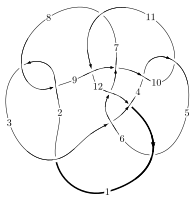
\includegraphics[width=112pt]{../../../GIT/diagram.site/Diagrams/png/1504_12a_0703.png}\\
\ \ \ A knot diagram\footnotemark}&
\allowdisplaybreaks
\textbf{Linearized knot diagam} \\
\cline{2-2}
 &
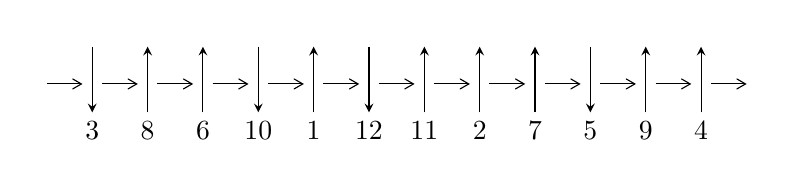
\begin{tikzpicture}[x=20pt, y=17pt]
	% nodes
	\node (C0) at (0, 0) {};
	\node (C1) at (1, 0) {};
	\node (C1U) at (1, +1) {};
	\node (C1D) at (1, -1) {3};

	\node (C2) at (2, 0) {};
	\node (C2U) at (2, +1) {};
	\node (C2D) at (2, -1) {8};

	\node (C3) at (3, 0) {};
	\node (C3U) at (3, +1) {};
	\node (C3D) at (3, -1) {6};

	\node (C4) at (4, 0) {};
	\node (C4U) at (4, +1) {};
	\node (C4D) at (4, -1) {10};

	\node (C5) at (5, 0) {};
	\node (C5U) at (5, +1) {};
	\node (C5D) at (5, -1) {1};

	\node (C6) at (6, 0) {};
	\node (C6U) at (6, +1) {};
	\node (C6D) at (6, -1) {12};

	\node (C7) at (7, 0) {};
	\node (C7U) at (7, +1) {};
	\node (C7D) at (7, -1) {11};

	\node (C8) at (8, 0) {};
	\node (C8U) at (8, +1) {};
	\node (C8D) at (8, -1) {2};

	\node (C9) at (9, 0) {};
	\node (C9U) at (9, +1) {};
	\node (C9D) at (9, -1) {7};

	\node (C10) at (10, 0) {};
	\node (C10U) at (10, +1) {};
	\node (C10D) at (10, -1) {5};

	\node (C11) at (11, 0) {};
	\node (C11U) at (11, +1) {};
	\node (C11D) at (11, -1) {9};

	\node (C12) at (12, 0) {};
	\node (C12U) at (12, +1) {};
	\node (C12D) at (12, -1) {4};
	\node (C13) at (13, 0) {};

	% arrows
	\draw[->,>={angle 60}]
	(C0) edge (C1) (C1) edge (C2) (C2) edge (C3) (C3) edge (C4) (C4) edge (C5) (C5) edge (C6) (C6) edge (C7) (C7) edge (C8) (C8) edge (C9) (C9) edge (C10) (C10) edge (C11) (C11) edge (C12) (C12) edge (C13) ;	\draw[->,>=stealth]
	(C1U) edge (C1D) (C2D) edge (C2U) (C3D) edge (C3U) (C4U) edge (C4D) (C5D) edge (C5U) (C6U) edge (C6D) (C7D) edge (C7U) (C8D) edge (C8U) (C9D) edge (C9U) (C10U) edge (C10D) (C11D) edge (C11U) (C12D) edge (C12U) ;
	\end{tikzpicture} \\
\hhline{~~} \\& 
\textbf{Solving Sequence} \\ \cline{2-2} 
 &
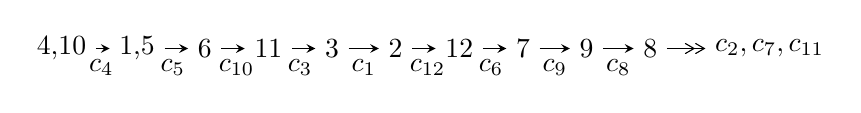
\begin{tikzpicture}[x=23pt, y=7pt]
	% node
	\node (A0) at (-1/8, 0) {4,10};
	\node (A1) at (17/16, 0) {1,5};
	\node (A2) at (17/8, 0) {6};
	\node (A3) at (25/8, 0) {11};
	\node (A4) at (33/8, 0) {3};
	\node (A5) at (41/8, 0) {2};
	\node (A6) at (49/8, 0) {12};
	\node (A7) at (57/8, 0) {7};
	\node (A8) at (65/8, 0) {9};
	\node (A9) at (73/8, 0) {8};
	\node (C1) at (1/2, -1) {$c_{4}$};
	\node (C2) at (13/8, -1) {$c_{5}$};
	\node (C3) at (21/8, -1) {$c_{10}$};
	\node (C4) at (29/8, -1) {$c_{3}$};
	\node (C5) at (37/8, -1) {$c_{1}$};
	\node (C6) at (45/8, -1) {$c_{12}$};
	\node (C7) at (53/8, -1) {$c_{6}$};
	\node (C8) at (61/8, -1) {$c_{9}$};
	\node (C9) at (69/8, -1) {$c_{8}$};
	\node (A10) at (11, 0) {$c_{2},c_{7},c_{11}$};

	% edge
	\draw[->,>=stealth]	
	(A0) edge (A1) (A1) edge (A2) (A2) edge (A3) (A3) edge (A4) (A4) edge (A5) (A5) edge (A6) (A6) edge (A7) (A7) edge (A8) (A8) edge (A9) ;
	\draw[->>,>={angle 60}]	
	(A9) edge (A10);
\end{tikzpicture} \\ 

\end{tabular} \\

\footnotetext{
The image of knot diagram is generated by the software ``\textbf{Draw programme}" developed by Andrew Bartholomew(\url{http://www.layer8.co.uk/maths/draw/index.htm\#Running-draw}), where we modified some parts for our purpose(\url{https://github.com/CATsTAILs/LinksPainter}).
}\phantom \\ \newline 
\centering \textbf{Ideals for irreducible components\footnotemark of $X_{\text{par}}$} 
 
\begin{align*}
I^u_{1}&=\langle 
-2.77114\times10^{184} u^{73}-8.17972\times10^{184} u^{72}+\cdots+7.24276\times10^{185} b-3.00731\times10^{186},\\
\phantom{I^u_{1}}&\phantom{= \langle  }-3.90392\times10^{186} u^{73}-9.58129\times10^{186} u^{72}+\cdots+3.62138\times10^{187} a-3.12806\times10^{188},\\
\phantom{I^u_{1}}&\phantom{= \langle  }u^{74}+3 u^{73}+\cdots+214 u+50\rangle \\
I^u_{2}&=\langle 
-6.87356\times10^{82} a u^{57}-2.10436\times10^{82} u^{57}+\cdots-1.52294\times10^{83} a-7.99339\times10^{82},\\
\phantom{I^u_{2}}&\phantom{= \langle  }-1.82997\times10^{84} a u^{57}+1.85456\times10^{84} u^{57}+\cdots-4.71969\times10^{84} a+5.09846\times10^{84},\;u^{58}+u^{57}+\cdots+2 u-1\rangle \\
I^u_{3}&=\langle 
-49666687602 u^{43}+10507987432 u^{42}+\cdots+285299162 b-67652116994,\\
\phantom{I^u_{3}}&\phantom{= \langle  }-787579015337 u^{43}-483419689064 u^{42}+\cdots+570598324 a+6927290387672,\\
\phantom{I^u_{3}}&\phantom{= \langle  }u^{44}-23 u^{42}+\cdots-102 u^2+4\rangle \\
\\
I^v_{1}&=\langle 
a,\;b-1,\;v+1\rangle \\
\end{align*}
\raggedright * 4 irreducible components of $\dim_{\mathbb{C}}=0$, with total 235 representations.\\
\footnotetext{All coefficients of polynomials are rational numbers. But the coefficients are sometimes approximated in decimal forms when there is not enough margin.}
\newpage
\renewcommand{\arraystretch}{1}
\centering \section*{I. $I^u_{1}= \langle -2.77\times10^{184} u^{73}-8.18\times10^{184} u^{72}+\cdots+7.24\times10^{185} b-3.01\times10^{186},\;-3.90\times10^{186} u^{73}-9.58\times10^{186} u^{72}+\cdots+3.62\times10^{187} a-3.13\times10^{188},\;u^{74}+3 u^{73}+\cdots+214 u+50 \rangle$}
\flushleft \textbf{(i) Arc colorings}\\
\begin{tabular}{m{7pt} m{180pt} m{7pt} m{180pt} }
\flushright $a_{4}=$&$\begin{pmatrix}1\\0\end{pmatrix}$ \\
\flushright $a_{10}=$&$\begin{pmatrix}0\\u\end{pmatrix}$ \\
\flushright $a_{1}=$&$\begin{pmatrix}0.107802 u^{73}+0.264576 u^{72}+\cdots+24.2519 u+8.63775\\0.0382609 u^{73}+0.112937 u^{72}+\cdots+12.7924 u+4.15217\end{pmatrix}$ \\
\flushright $a_{5}=$&$\begin{pmatrix}1\\u^2\end{pmatrix}$ \\
\flushright $a_{6}=$&$\begin{pmatrix}-0.0174281 u^{73}+0.0100093 u^{72}+\cdots+5.03284 u+4.77196\\0.0332921 u^{73}+0.0750533 u^{72}+\cdots+6.06430 u+2.23615\end{pmatrix}$ \\
\flushright $a_{11}=$&$\begin{pmatrix}- u\\- u^3+u\end{pmatrix}$ \\
\flushright $a_{3}=$&$\begin{pmatrix}0.0978843 u^{73}+0.202898 u^{72}+\cdots+16.0050 u+4.42091\\-0.0116068 u^{73}-0.0547438 u^{72}+\cdots-6.38601 u-2.84452\end{pmatrix}$ \\
\flushright $a_{2}=$&$\begin{pmatrix}-0.0552379 u^{73}-0.170989 u^{72}+\cdots-21.5165 u-7.21064\\0.0266858 u^{73}+0.0963030 u^{72}+\cdots+9.95127 u+3.43602\end{pmatrix}$ \\
\flushright $a_{12}=$&$\begin{pmatrix}0.0695411 u^{73}+0.151639 u^{72}+\cdots+11.4595 u+4.48558\\0.0382609 u^{73}+0.112937 u^{72}+\cdots+12.7924 u+4.15217\end{pmatrix}$ \\
\flushright $a_{7}=$&$\begin{pmatrix}-0.0830434 u^{73}-0.210869 u^{72}+\cdots-20.1108 u-4.97888\\0.0569840 u^{73}+0.120041 u^{72}+\cdots+10.3962 u+3.47705\end{pmatrix}$ \\
\flushright $a_{9}=$&$\begin{pmatrix}0.114207 u^{73}+0.198009 u^{72}+\cdots+8.85708 u+1.31279\\-0.0212613 u^{73}+0.00813017 u^{72}+\cdots+4.74494 u+2.41140\end{pmatrix}$ \\
\flushright $a_{8}=$&$\begin{pmatrix}-0.0897966 u^{73}-0.235013 u^{72}+\cdots-22.2995 u-5.77312\\0.0766086 u^{73}+0.164871 u^{72}+\cdots+13.7536 u+4.46546\end{pmatrix}$\\&\end{tabular}
\flushleft \textbf{(ii) Obstruction class $= -1$}\\~\\
\flushleft \textbf{(iii) Cusp Shapes $= -0.347145 u^{73}-0.680756 u^{72}+\cdots-47.9021 u-9.04265$}\\~\\
\newpage\renewcommand{\arraystretch}{1}
\flushleft \textbf{(iv) u-Polynomials at the component}\newline \\
\begin{tabular}{m{50pt}|m{274pt}}
Crossings & \hspace{64pt}u-Polynomials at each crossing \\
\hline $$\begin{aligned}c_{1}\end{aligned}$$&$\begin{aligned}
&u^{74}+27 u^{73}+\cdots+5620 u+676
\end{aligned}$\\
\hline $$\begin{aligned}c_{2},c_{8}\end{aligned}$$&$\begin{aligned}
&u^{74}+3 u^{73}+\cdots+198 u+26
\end{aligned}$\\
\hline $$\begin{aligned}c_{3},c_{11}\end{aligned}$$&$\begin{aligned}
&u^{74}+u^{73}+\cdots-4 u+1
\end{aligned}$\\
\hline $$\begin{aligned}c_{4},c_{10}\end{aligned}$$&$\begin{aligned}
&u^{74}-3 u^{73}+\cdots-214 u+50
\end{aligned}$\\
\hline $$\begin{aligned}c_{5},c_{7}\end{aligned}$$&$\begin{aligned}
&u^{74}- u^{73}+\cdots-16 u+1
\end{aligned}$\\
\hline $$\begin{aligned}c_{6}\end{aligned}$$&$\begin{aligned}
&u^{74}-3 u^{73}+\cdots-71216 u+11944
\end{aligned}$\\
\hline $$\begin{aligned}c_{9},c_{12}\end{aligned}$$&$\begin{aligned}
&u^{74}+5 u^{73}+\cdots+2 u+1
\end{aligned}$\\
\hline
\end{tabular}\\~\\
\newpage\renewcommand{\arraystretch}{1}
\flushleft \textbf{(v) Riley Polynomials at the component}\newline \\
\begin{tabular}{m{50pt}|m{274pt}}
Crossings & \hspace{64pt}Riley Polynomials at each crossing \\
\hline $$\begin{aligned}c_{1}\end{aligned}$$&$\begin{aligned}
&y^{74}+27 y^{73}+\cdots+8851216 y+456976
\end{aligned}$\\
\hline $$\begin{aligned}c_{2},c_{8}\end{aligned}$$&$\begin{aligned}
&y^{74}+27 y^{73}+\cdots+5620 y+676
\end{aligned}$\\
\hline $$\begin{aligned}c_{3},c_{11}\end{aligned}$$&$\begin{aligned}
&y^{74}-13 y^{73}+\cdots-4 y+1
\end{aligned}$\\
\hline $$\begin{aligned}c_{4},c_{10}\end{aligned}$$&$\begin{aligned}
&y^{74}-29 y^{73}+\cdots+11604 y+2500
\end{aligned}$\\
\hline $$\begin{aligned}c_{5},c_{7}\end{aligned}$$&$\begin{aligned}
&y^{74}+y^{73}+\cdots-84 y+1
\end{aligned}$\\
\hline $$\begin{aligned}c_{6}\end{aligned}$$&$\begin{aligned}
&y^{74}- y^{73}+\cdots+999177664 y+142659136
\end{aligned}$\\
\hline $$\begin{aligned}c_{9},c_{12}\end{aligned}$$&$\begin{aligned}
&y^{74}+17 y^{73}+\cdots+38 y+1
\end{aligned}$\\
\hline
\end{tabular}\\~\\
\newpage\flushleft \textbf{(vi) Complex Volumes and Cusp Shapes}
$$\begin{array}{c|c|c}  
\text{Solutions to }I^u_{1}& \I (\text{vol} + \sqrt{-1}CS) & \text{Cusp shape}\\
 \hline 
\begin{aligned}
u &= -0.909614 + 0.396950 I \\
a &= -1.31457 + 0.85012 I \\
b &= -0.38186 + 1.47154 I\end{aligned}
 & \phantom{-}0.22853 - 2.72746 I & \phantom{-0.000000 -}0. + 8.02021 I \\ \hline\begin{aligned}
u &= -0.909614 - 0.396950 I \\
a &= -1.31457 - 0.85012 I \\
b &= -0.38186 - 1.47154 I\end{aligned}
 & \phantom{-}0.22853 + 2.72746 I & \phantom{-0.000000 } 0. - 8.02021 I \\ \hline\begin{aligned}
u &= -0.914825 + 0.342039 I \\
a &= \phantom{-}0.57785 + 2.25113 I \\
b &= \phantom{-}1.97680 + 0.53701 I\end{aligned}
 & -3.78901 + 1.40165 I & -16.4410 - 0.7863 I \\ \hline\begin{aligned}
u &= -0.914825 - 0.342039 I \\
a &= \phantom{-}0.57785 - 2.25113 I \\
b &= \phantom{-}1.97680 - 0.53701 I\end{aligned}
 & -3.78901 - 1.40165 I & -16.4410 + 0.7863 I \\ \hline\begin{aligned}
u &= -0.156031 + 0.945245 I \\
a &= -0.313085 + 0.209961 I \\
b &= \phantom{-}0.996616 - 0.878583 I\end{aligned}
 & -1.52890 - 7.84005 I & \phantom{-}1.78951 + 8.16900 I \\ \hline\begin{aligned}
u &= -0.156031 - 0.945245 I \\
a &= -0.313085 - 0.209961 I \\
b &= \phantom{-}0.996616 + 0.878583 I\end{aligned}
 & -1.52890 + 7.84005 I & \phantom{-}1.78951 - 8.16900 I \\ \hline\begin{aligned}
u &= \phantom{-}0.839218 + 0.444879 I \\
a &= -0.548436 - 0.741129 I \\
b &= \phantom{-}0.622338 - 0.358532 I\end{aligned}
 & -1.15865 - 1.75347 I & \phantom{-}0.42379 + 2.04993 I \\ \hline\begin{aligned}
u &= \phantom{-}0.839218 - 0.444879 I \\
a &= -0.548436 + 0.741129 I \\
b &= \phantom{-}0.622338 + 0.358532 I\end{aligned}
 & -1.15865 + 1.75347 I & \phantom{-}0.42379 - 2.04993 I \\ \hline\begin{aligned}
u &= \phantom{-}1.044270 + 0.363592 I \\
a &= -0.73827 - 1.76439 I \\
b &= \phantom{-}0.667890 - 1.080670 I\end{aligned}
 & -1.411110 - 0.014479 I & \phantom{-0.000000 } 0 \\ \hline\begin{aligned}
u &= \phantom{-}1.044270 - 0.363592 I \\
a &= -0.73827 + 1.76439 I \\
b &= \phantom{-}0.667890 + 1.080670 I\end{aligned}
 & -1.411110 + 0.014479 I & \phantom{-0.000000 } 0\\
 \hline 
 \end{array}$$\newpage$$\begin{array}{c|c|c}  
\text{Solutions to }I^u_{1}& \I (\text{vol} + \sqrt{-1}CS) & \text{Cusp shape}\\
 \hline 
\begin{aligned}
u &= \phantom{-}0.860878 + 0.727657 I \\
a &= -0.618550 - 0.759462 I \\
b &= \phantom{-}0.600060 - 0.732713 I\end{aligned}
 & -0.84983 - 1.69851 I & \phantom{-0.000000 } 0 \\ \hline\begin{aligned}
u &= \phantom{-}0.860878 - 0.727657 I \\
a &= -0.618550 + 0.759462 I \\
b &= \phantom{-}0.600060 + 0.732713 I\end{aligned}
 & -0.84983 + 1.69851 I & \phantom{-0.000000 } 0 \\ \hline\begin{aligned}
u &= \phantom{-}1.072970 + 0.375190 I \\
a &= -0.854523 - 0.536536 I \\
b &= \phantom{-}0.297599 - 0.246377 I\end{aligned}
 & -0.86822 - 1.28553 I & \phantom{-0.000000 } 0 \\ \hline\begin{aligned}
u &= \phantom{-}1.072970 - 0.375190 I \\
a &= -0.854523 + 0.536536 I \\
b &= \phantom{-}0.297599 + 0.246377 I\end{aligned}
 & -0.86822 + 1.28553 I & \phantom{-0.000000 } 0 \\ \hline\begin{aligned}
u &= -1.012580 + 0.530794 I \\
a &= \phantom{-}1.06495 - 1.30603 I \\
b &= -0.129319 - 1.382060 I\end{aligned}
 & -0.42776 + 6.41562 I & \phantom{-0.000000 } 0 \\ \hline\begin{aligned}
u &= -1.012580 - 0.530794 I \\
a &= \phantom{-}1.06495 + 1.30603 I \\
b &= -0.129319 + 1.382060 I\end{aligned}
 & -0.42776 - 6.41562 I & \phantom{-0.000000 } 0 \\ \hline\begin{aligned}
u &= -1.057450 + 0.447518 I \\
a &= -0.03575 - 2.02403 I \\
b &= -0.334913 - 0.958480 I\end{aligned}
 & -0.65318 + 5.68113 I & \phantom{-0.000000 } 0 \\ \hline\begin{aligned}
u &= -1.057450 - 0.447518 I \\
a &= -0.03575 + 2.02403 I \\
b &= -0.334913 + 0.958480 I\end{aligned}
 & -0.65318 - 5.68113 I & \phantom{-0.000000 } 0 \\ \hline\begin{aligned}
u &= -0.836971 + 0.102898 I \\
a &= \phantom{-}0.83457 - 1.80288 I \\
b &= -0.812591 - 0.770221 I\end{aligned}
 & \phantom{-}0.46152 + 4.69310 I & \phantom{-}4.12938 - 8.24884 I \\ \hline\begin{aligned}
u &= -0.836971 - 0.102898 I \\
a &= \phantom{-}0.83457 + 1.80288 I \\
b &= -0.812591 + 0.770221 I\end{aligned}
 & \phantom{-}0.46152 - 4.69310 I & \phantom{-}4.12938 + 8.24884 I\\
 \hline 
 \end{array}$$\newpage$$\begin{array}{c|c|c}  
\text{Solutions to }I^u_{1}& \I (\text{vol} + \sqrt{-1}CS) & \text{Cusp shape}\\
 \hline 
\begin{aligned}
u &= \phantom{-}0.016940 + 1.158480 I \\
a &= -0.066432 - 0.683445 I \\
b &= -0.028731 + 0.330331 I\end{aligned}
 & \phantom{-}5.48738 - 2.71261 I & \phantom{-0.000000 } 0 \\ \hline\begin{aligned}
u &= \phantom{-}0.016940 - 1.158480 I \\
a &= -0.066432 + 0.683445 I \\
b &= -0.028731 - 0.330331 I\end{aligned}
 & \phantom{-}5.48738 + 2.71261 I & \phantom{-0.000000 } 0 \\ \hline\begin{aligned}
u &= \phantom{-}1.025760 + 0.541737 I \\
a &= \phantom{-}0.41059 + 2.11387 I \\
b &= -1.52964 + 1.41048 I\end{aligned}
 & \phantom{-}1.48385 - 8.36167 I & \phantom{-0.000000 } 0 \\ \hline\begin{aligned}
u &= \phantom{-}1.025760 - 0.541737 I \\
a &= \phantom{-}0.41059 - 2.11387 I \\
b &= -1.52964 - 1.41048 I\end{aligned}
 & \phantom{-}1.48385 + 8.36167 I & \phantom{-0.000000 } 0 \\ \hline\begin{aligned}
u &= \phantom{-}1.085750 + 0.485137 I \\
a &= -0.08294 - 2.07700 I \\
b &= \phantom{-}0.349227 - 0.934147 I\end{aligned}
 & -1.60589 - 11.15020 I & \phantom{-0.000000 } 0 \\ \hline\begin{aligned}
u &= \phantom{-}1.085750 - 0.485137 I \\
a &= -0.08294 + 2.07700 I \\
b &= \phantom{-}0.349227 + 0.934147 I\end{aligned}
 & -1.60589 + 11.15020 I & \phantom{-0.000000 } 0 \\ \hline\begin{aligned}
u &= -1.066850 + 0.539758 I \\
a &= \phantom{-}0.893161 - 0.801409 I \\
b &= -0.159467 - 0.448777 I\end{aligned}
 & -5.45308 + 1.99266 I & \phantom{-0.000000 } 0 \\ \hline\begin{aligned}
u &= -1.066850 - 0.539758 I \\
a &= \phantom{-}0.893161 + 0.801409 I \\
b &= -0.159467 + 0.448777 I\end{aligned}
 & -5.45308 - 1.99266 I & \phantom{-0.000000 } 0 \\ \hline\begin{aligned}
u &= \phantom{-}0.533812 + 0.595532 I \\
a &= -0.507118 + 1.037650 I \\
b &= -1.34739 - 0.86281 I\end{aligned}
 & \phantom{-}2.95358 + 3.82344 I & \phantom{-}8.69107 - 9.53262 I \\ \hline\begin{aligned}
u &= \phantom{-}0.533812 - 0.595532 I \\
a &= -0.507118 - 1.037650 I \\
b &= -1.34739 + 0.86281 I\end{aligned}
 & \phantom{-}2.95358 - 3.82344 I & \phantom{-}8.69107 + 9.53262 I\\
 \hline 
 \end{array}$$\newpage$$\begin{array}{c|c|c}  
\text{Solutions to }I^u_{1}& \I (\text{vol} + \sqrt{-1}CS) & \text{Cusp shape}\\
 \hline 
\begin{aligned}
u &= -0.308390 + 0.731898 I \\
a &= -0.364711 - 0.092810 I \\
b &= -0.421888 + 0.506910 I\end{aligned}
 & \phantom{-}1.14192 - 0.87156 I & \phantom{-}5.34852 + 4.41242 I \\ \hline\begin{aligned}
u &= -0.308390 - 0.731898 I \\
a &= -0.364711 + 0.092810 I \\
b &= -0.421888 - 0.506910 I\end{aligned}
 & \phantom{-}1.14192 + 0.87156 I & \phantom{-}5.34852 - 4.41242 I \\ \hline\begin{aligned}
u &= \phantom{-}1.020790 + 0.657917 I \\
a &= \phantom{-}0.833528 + 0.270019 I \\
b &= \phantom{-}0.626919 + 1.126860 I\end{aligned}
 & -1.53010 - 3.80254 I & \phantom{-0.000000 } 0 \\ \hline\begin{aligned}
u &= \phantom{-}1.020790 - 0.657917 I \\
a &= \phantom{-}0.833528 - 0.270019 I \\
b &= \phantom{-}0.626919 - 1.126860 I\end{aligned}
 & -1.53010 + 3.80254 I & \phantom{-0.000000 } 0 \\ \hline\begin{aligned}
u &= -1.148110 + 0.431399 I \\
a &= \phantom{-}0.977559 - 0.597525 I \\
b &= -0.206503 - 0.254163 I\end{aligned}
 & -1.89189 - 3.73040 I & \phantom{-0.000000 } 0 \\ \hline\begin{aligned}
u &= -1.148110 - 0.431399 I \\
a &= \phantom{-}0.977559 + 0.597525 I \\
b &= -0.206503 + 0.254163 I\end{aligned}
 & -1.89189 + 3.73040 I & \phantom{-0.000000 } 0 \\ \hline\begin{aligned}
u &= -0.238711 + 1.208710 I \\
a &= -0.202115 - 0.121447 I \\
b &= -0.187999 + 0.669054 I\end{aligned}
 & \phantom{-}1.36765 - 0.67560 I & \phantom{-0.000000 } 0 \\ \hline\begin{aligned}
u &= -0.238711 - 1.208710 I \\
a &= -0.202115 + 0.121447 I \\
b &= -0.187999 - 0.669054 I\end{aligned}
 & \phantom{-}1.36765 + 0.67560 I & \phantom{-0.000000 } 0 \\ \hline\begin{aligned}
u &= \phantom{-}1.154100 + 0.436756 I \\
a &= -0.29573 - 1.81016 I \\
b &= \phantom{-}0.420473 - 0.969989 I\end{aligned}
 & -5.95591 - 5.60935 I & \phantom{-0.000000 } 0 \\ \hline\begin{aligned}
u &= \phantom{-}1.154100 - 0.436756 I \\
a &= -0.29573 + 1.81016 I \\
b &= \phantom{-}0.420473 + 0.969989 I\end{aligned}
 & -5.95591 + 5.60935 I & \phantom{-0.000000 } 0\\
 \hline 
 \end{array}$$\newpage$$\begin{array}{c|c|c}  
\text{Solutions to }I^u_{1}& \I (\text{vol} + \sqrt{-1}CS) & \text{Cusp shape}\\
 \hline 
\begin{aligned}
u &= \phantom{-}0.471889 + 1.146720 I \\
a &= -0.0814819 + 0.0066989 I \\
b &= -1.00813 - 0.99688 I\end{aligned}
 & \phantom{-}6.01642 + 8.62957 I & \phantom{-0.000000 } 0 \\ \hline\begin{aligned}
u &= \phantom{-}0.471889 - 1.146720 I \\
a &= -0.0814819 - 0.0066989 I \\
b &= -1.00813 + 0.99688 I\end{aligned}
 & \phantom{-}6.01642 - 8.62957 I & \phantom{-0.000000 } 0 \\ \hline\begin{aligned}
u &= -1.244920 + 0.264711 I \\
a &= -0.190377 - 1.363030 I \\
b &= -0.384430 - 1.068030 I\end{aligned}
 & -2.92533 + 4.99049 I & \phantom{-0.000000 } 0 \\ \hline\begin{aligned}
u &= -1.244920 - 0.264711 I \\
a &= -0.190377 + 1.363030 I \\
b &= -0.384430 + 1.068030 I\end{aligned}
 & -2.92533 - 4.99049 I & \phantom{-0.000000 } 0 \\ \hline\begin{aligned}
u &= -0.431800 + 1.236090 I \\
a &= \phantom{-}0.0261358 - 0.0618161 I \\
b &= \phantom{-}0.984830 - 0.995193 I\end{aligned}
 & \phantom{-}4.6749 - 14.7050 I & \phantom{-0.000000 } 0 \\ \hline\begin{aligned}
u &= -0.431800 - 1.236090 I \\
a &= \phantom{-}0.0261358 + 0.0618161 I \\
b &= \phantom{-}0.984830 + 0.995193 I\end{aligned}
 & \phantom{-}4.6749 + 14.7050 I & \phantom{-0.000000 } 0 \\ \hline\begin{aligned}
u &= -0.629169 + 0.236880 I \\
a &= \phantom{-}0.65931 + 2.02972 I \\
b &= -0.748058 + 0.680934 I\end{aligned}
 & \phantom{-}1.11590 - 2.39492 I & \phantom{-}3.38619 + 4.33941 I \\ \hline\begin{aligned}
u &= -0.629169 - 0.236880 I \\
a &= \phantom{-}0.65931 - 2.02972 I \\
b &= -0.748058 - 0.680934 I\end{aligned}
 & \phantom{-}1.11590 + 2.39492 I & \phantom{-}3.38619 - 4.33941 I \\ \hline\begin{aligned}
u &= -1.201760 + 0.569657 I \\
a &= -0.24781 + 1.72565 I \\
b &= \phantom{-}1.31232 + 1.15494 I\end{aligned}
 & -4.61734 + 13.19020 I & \phantom{-0.000000 } 0 \\ \hline\begin{aligned}
u &= -1.201760 - 0.569657 I \\
a &= -0.24781 - 1.72565 I \\
b &= \phantom{-}1.31232 - 1.15494 I\end{aligned}
 & -4.61734 - 13.19020 I & \phantom{-0.000000 } 0\\
 \hline 
 \end{array}$$\newpage$$\begin{array}{c|c|c}  
\text{Solutions to }I^u_{1}& \I (\text{vol} + \sqrt{-1}CS) & \text{Cusp shape}\\
 \hline 
\begin{aligned}
u &= -1.119050 + 0.725619 I \\
a &= \phantom{-}0.478422 - 0.920331 I \\
b &= -0.470840 - 0.896553 I\end{aligned}
 & -1.02125 + 6.53391 I & \phantom{-0.000000 } 0 \\ \hline\begin{aligned}
u &= -1.119050 - 0.725619 I \\
a &= \phantom{-}0.478422 + 0.920331 I \\
b &= -0.470840 + 0.896553 I\end{aligned}
 & -1.02125 - 6.53391 I & \phantom{-0.000000 } 0 \\ \hline\begin{aligned}
u &= -0.469402 + 0.468395 I \\
a &= \phantom{-}1.43700 - 0.99968 I \\
b &= \phantom{-}0.629288 + 0.085931 I\end{aligned}
 & \phantom{-}0.51998 + 7.85032 I & \phantom{-}2.36500 - 7.37361 I \\ \hline\begin{aligned}
u &= -0.469402 - 0.468395 I \\
a &= \phantom{-}1.43700 + 0.99968 I \\
b &= \phantom{-}0.629288 - 0.085931 I\end{aligned}
 & \phantom{-}0.51998 - 7.85032 I & \phantom{-}2.36500 + 7.37361 I \\ \hline\begin{aligned}
u &= \phantom{-}0.208263 + 0.596482 I \\
a &= -1.285370 - 0.342537 I \\
b &= -0.512967 + 0.281947 I\end{aligned}
 & \phantom{-}1.97475 - 2.48823 I & \phantom{-}5.74600 + 3.53308 I \\ \hline\begin{aligned}
u &= \phantom{-}0.208263 - 0.596482 I \\
a &= -1.285370 + 0.342537 I \\
b &= -0.512967 - 0.281947 I\end{aligned}
 & \phantom{-}1.97475 + 2.48823 I & \phantom{-}5.74600 - 3.53308 I \\ \hline\begin{aligned}
u &= \phantom{-}0.463250 + 0.386578 I \\
a &= -0.27743 + 2.01381 I \\
b &= \phantom{-}0.712206 + 0.654034 I\end{aligned}
 & \phantom{-}0.41291 + 7.22676 I & \phantom{-}2.21127 - 10.05995 I \\ \hline\begin{aligned}
u &= \phantom{-}0.463250 - 0.386578 I \\
a &= -0.27743 - 2.01381 I \\
b &= \phantom{-}0.712206 - 0.654034 I\end{aligned}
 & \phantom{-}0.41291 - 7.22676 I & \phantom{-}2.21127 + 10.05995 I \\ \hline\begin{aligned}
u &= \phantom{-}0.095915 + 0.580931 I \\
a &= \phantom{-}0.225917 + 0.767444 I \\
b &= \phantom{-}0.488108 + 0.617790 I\end{aligned}
 & -2.97292 + 1.62134 I & -2.53607 - 4.07358 I \\ \hline\begin{aligned}
u &= \phantom{-}0.095915 - 0.580931 I \\
a &= \phantom{-}0.225917 - 0.767444 I \\
b &= \phantom{-}0.488108 - 0.617790 I\end{aligned}
 & -2.97292 - 1.62134 I & -2.53607 + 4.07358 I\\
 \hline 
 \end{array}$$\newpage$$\begin{array}{c|c|c}  
\text{Solutions to }I^u_{1}& \I (\text{vol} + \sqrt{-1}CS) & \text{Cusp shape}\\
 \hline 
\begin{aligned}
u &= \phantom{-}1.22021 + 0.72285 I \\
a &= \phantom{-}0.38795 + 1.58435 I \\
b &= -1.18281 + 1.18650 I\end{aligned}
 & \phantom{-}3.5916 - 15.2618 I & \phantom{-0.000000 } 0 \\ \hline\begin{aligned}
u &= \phantom{-}1.22021 - 0.72285 I \\
a &= \phantom{-}0.38795 - 1.58435 I \\
b &= -1.18281 - 1.18650 I\end{aligned}
 & \phantom{-}3.5916 + 15.2618 I & \phantom{-0.000000 } 0 \\ \hline\begin{aligned}
u &= \phantom{-}1.41967 + 0.19256 I \\
a &= \phantom{-}0.493968 + 0.886865 I \\
b &= \phantom{-}0.420556 + 1.156770 I\end{aligned}
 & -7.02583 + 3.28946 I & \phantom{-0.000000 } 0 \\ \hline\begin{aligned}
u &= \phantom{-}1.41967 - 0.19256 I \\
a &= \phantom{-}0.493968 - 0.886865 I \\
b &= \phantom{-}0.420556 - 1.156770 I\end{aligned}
 & -7.02583 - 3.28946 I & \phantom{-0.000000 } 0 \\ \hline\begin{aligned}
u &= -1.27001 + 0.73550 I \\
a &= -0.35927 + 1.54105 I \\
b &= \phantom{-}1.17202 + 1.15521 I\end{aligned}
 & \phantom{-}1.9496 + 21.6262 I & \phantom{-0.000000 } 0 \\ \hline\begin{aligned}
u &= -1.27001 - 0.73550 I \\
a &= -0.35927 - 1.54105 I \\
b &= \phantom{-}1.17202 - 1.15521 I\end{aligned}
 & \phantom{-}1.9496 - 21.6262 I & \phantom{-0.000000 } 0 \\ \hline\begin{aligned}
u &= -1.52992 + 0.27858 I \\
a &= -0.122728 - 1.027730 I \\
b &= -0.439615 - 1.094750 I\end{aligned}
 & -2.64674 + 4.78715 I & \phantom{-0.000000 } 0 \\ \hline\begin{aligned}
u &= -1.52992 - 0.27858 I \\
a &= -0.122728 + 1.027730 I \\
b &= -0.439615 + 1.094750 I\end{aligned}
 & -2.64674 - 4.78715 I & \phantom{-0.000000 } 0 \\ \hline\begin{aligned}
u &= -0.079882 + 0.380032 I \\
a &= -0.609520 - 0.407700 I \\
b &= \phantom{-}0.094707 + 0.887383 I\end{aligned}
 & \phantom{-}1.30410 - 2.82260 I & \phantom{-}2.38703 + 2.73836 I \\ \hline\begin{aligned}
u &= -0.079882 - 0.380032 I \\
a &= -0.609520 + 0.407700 I \\
b &= \phantom{-}0.094707 - 0.887383 I\end{aligned}
 & \phantom{-}1.30410 + 2.82260 I & \phantom{-}2.38703 - 2.73836 I\\
 \hline 
 \end{array}$$\newpage$$\begin{array}{c|c|c}  
\text{Solutions to }I^u_{1}& \I (\text{vol} + \sqrt{-1}CS) & \text{Cusp shape}\\
 \hline 
\begin{aligned}
u &= \phantom{-}1.67121 + 0.12671 I \\
a &= \phantom{-}0.202894 - 0.909208 I \\
b &= \phantom{-}0.445070 - 1.122660 I\end{aligned}
 & -3.83527 - 9.66068 I & \phantom{-0.000000 } 0 \\ \hline\begin{aligned}
u &= \phantom{-}1.67121 - 0.12671 I \\
a &= \phantom{-}0.202894 + 0.909208 I \\
b &= \phantom{-}0.445070 + 1.122660 I\end{aligned}
 & -3.83527 + 9.66068 I & \phantom{-0.000000 } 0 \\ \hline\begin{aligned}
u &= -0.07945 + 1.67803 I \\
a &= -0.0275868 + 0.0547943 I \\
b &= -0.029860 + 0.867336 I\end{aligned}
 & \phantom{-}3.50160 + 2.46193 I & \phantom{-0.000000 } 0 \\ \hline\begin{aligned}
u &= -0.07945 - 1.67803 I \\
a &= -0.0275868 - 0.0547943 I \\
b &= -0.029860 - 0.867336 I\end{aligned}
 & \phantom{-}3.50160 - 2.46193 I & \phantom{-0.000000 } 0\\
 \hline 
 \end{array}$$\newpage\newpage\renewcommand{\arraystretch}{1}
\centering \section*{II. $I^u_{2}= \langle -6.87\times10^{82} a u^{57}-2.10\times10^{82} u^{57}+\cdots-1.52\times10^{83} a-7.99\times10^{82},\;-1.83\times10^{84} a u^{57}+1.85\times10^{84} u^{57}+\cdots-4.72\times10^{84} a+5.10\times10^{84},\;u^{58}+u^{57}+\cdots+2 u-1 \rangle$}
\flushleft \textbf{(i) Arc colorings}\\
\begin{tabular}{m{7pt} m{180pt} m{7pt} m{180pt} }
\flushright $a_{4}=$&$\begin{pmatrix}1\\0\end{pmatrix}$ \\
\flushright $a_{10}=$&$\begin{pmatrix}0\\u\end{pmatrix}$ \\
\flushright $a_{1}=$&$\begin{pmatrix}a\\3.94498 a u^{57}+1.20777 u^{57}+\cdots+8.74070 a+4.58770\end{pmatrix}$ \\
\flushright $a_{5}=$&$\begin{pmatrix}1\\u^2\end{pmatrix}$ \\
\flushright $a_{6}=$&$\begin{pmatrix}11.7169 a u^{57}-25.6973 u^{57}+\cdots+34.7947 a-81.3867\\-3.44910 a u^{57}-9.14563 u^{57}+\cdots-7.51696 a-29.9963\end{pmatrix}$ \\
\flushright $a_{11}=$&$\begin{pmatrix}- u\\- u^3+u\end{pmatrix}$ \\
\flushright $a_{3}=$&$\begin{pmatrix}13.0375 a u^{57}+2.87073 u^{57}+\cdots+32.4685 a+12.1830\\0.641108 a u^{57}+30.3518 u^{57}+\cdots-0.00590775 a+91.5551\end{pmatrix}$ \\
\flushright $a_{2}=$&$\begin{pmatrix}-4.61184 a u^{57}-1.77005 u^{57}+\cdots-23.6676 a+11.0247\\-2.57353 a u^{57}+1.27800 u^{57}+\cdots-6.67995 a-7.63184\end{pmatrix}$ \\
\flushright $a_{12}=$&$\begin{pmatrix}-3.94498 a u^{57}-1.20777 u^{57}+\cdots-7.74070 a-4.58770\\3.94498 a u^{57}+1.20777 u^{57}+\cdots+8.74070 a+4.58770\end{pmatrix}$ \\
\flushright $a_{7}=$&$\begin{pmatrix}-8.74070 a u^{57}+0.283128 u^{57}+\cdots-17.6876 a-7.07158\\-1.39456 a u^{57}-35.1260 u^{57}+\cdots-3.94498 a-104.311\end{pmatrix}$ \\
\flushright $a_{9}=$&$\begin{pmatrix}7.46877 a u^{57}-2.82013 u^{57}+\cdots+19.3491 a-9.27593\\0.116447 a u^{57}+5.74680 u^{57}+\cdots+1.69257 a+11.6060\end{pmatrix}$ \\
\flushright $a_{8}=$&$\begin{pmatrix}-10.1353 a u^{57}-3.00479 u^{57}+\cdots-21.6326 a-18.7884\\0.641108 a u^{57}-33.1069 u^{57}+\cdots-0.00590775 a-94.2059\end{pmatrix}$\\&\end{tabular}
\flushleft \textbf{(ii) Obstruction class $= -1$}\\~\\
\flushleft \textbf{(iii) Cusp Shapes $= -129.417 u^{57}-187.821 u^{56}+\cdots-119.252 u-320.679$}\\~\\
\newpage\renewcommand{\arraystretch}{1}
\flushleft \textbf{(iv) u-Polynomials at the component}\newline \\
\begin{tabular}{m{50pt}|m{274pt}}
Crossings & \hspace{64pt}u-Polynomials at each crossing \\
\hline $$\begin{aligned}c_{1}\end{aligned}$$&$\begin{aligned}
&(u^{58}+24 u^{57}+\cdots+31 u+1)^{2}
\end{aligned}$\\
\hline $$\begin{aligned}c_{2}\end{aligned}$$&$\begin{aligned}
&(u^{58}+12 u^{56}+\cdots+9 u-1)^{2}
\end{aligned}$\\
\hline $$\begin{aligned}c_{3}\end{aligned}$$&$\begin{aligned}
&u^{116}+25 u^{115}+\cdots-117584 u-11337
\end{aligned}$\\
\hline $$\begin{aligned}c_{4}\end{aligned}$$&$\begin{aligned}
&(u^{58}- u^{57}+\cdots-2 u-1)^{2}
\end{aligned}$\\
\hline $$\begin{aligned}c_{5}\end{aligned}$$&$\begin{aligned}
&- u^{116}+24 u^{114}+\cdots-91697 u+9341
\end{aligned}$\\
\hline $$\begin{aligned}c_{6}\end{aligned}$$&$\begin{aligned}
&(u^{58}+19 u^{56}+\cdots+2418 u-169)^{2}
\end{aligned}$\\
\hline $$\begin{aligned}c_{7}\end{aligned}$$&$\begin{aligned}
&u^{116}-24 u^{114}+\cdots-91697 u-9341
\end{aligned}$\\
\hline $$\begin{aligned}c_{8}\end{aligned}$$&$\begin{aligned}
&(u^{58}+12 u^{56}+\cdots-9 u-1)^{2}
\end{aligned}$\\
\hline $$\begin{aligned}c_{9},c_{12}\end{aligned}$$&$\begin{aligned}
&u^{116}-11 u^{115}+\cdots-10 u+3
\end{aligned}$\\
\hline $$\begin{aligned}c_{10}\end{aligned}$$&$\begin{aligned}
&(u^{58}+u^{57}+\cdots+2 u-1)^{2}
\end{aligned}$\\
\hline $$\begin{aligned}c_{11}\end{aligned}$$&$\begin{aligned}
&- u^{116}+25 u^{115}+\cdots-117584 u+11337
\end{aligned}$\\
\hline
\end{tabular}\\~\\
\newpage\renewcommand{\arraystretch}{1}
\flushleft \textbf{(v) Riley Polynomials at the component}\newline \\
\begin{tabular}{m{50pt}|m{274pt}}
Crossings & \hspace{64pt}Riley Polynomials at each crossing \\
\hline $$\begin{aligned}c_{1}\end{aligned}$$&$\begin{aligned}
&(y^{58}+28 y^{57}+\cdots+99 y+1)^{2}
\end{aligned}$\\
\hline $$\begin{aligned}c_{2},c_{8}\end{aligned}$$&$\begin{aligned}
&(y^{58}+24 y^{57}+\cdots+31 y+1)^{2}
\end{aligned}$\\
\hline $$\begin{aligned}c_{3},c_{11}\end{aligned}$$&$\begin{aligned}
&y^{116}-41 y^{115}+\cdots-774026392 y+128527569
\end{aligned}$\\
\hline $$\begin{aligned}c_{4},c_{10}\end{aligned}$$&$\begin{aligned}
&(y^{58}-43 y^{57}+\cdots-36 y+1)^{2}
\end{aligned}$\\
\hline $$\begin{aligned}c_{5},c_{7}\end{aligned}$$&$\begin{aligned}
&y^{116}-48 y^{115}+\cdots-2631435723 y+87254281
\end{aligned}$\\
\hline $$\begin{aligned}c_{6}\end{aligned}$$&$\begin{aligned}
&(y^{58}+38 y^{57}+\cdots-3832244 y+28561)^{2}
\end{aligned}$\\
\hline $$\begin{aligned}c_{9},c_{12}\end{aligned}$$&$\begin{aligned}
&y^{116}-59 y^{115}+\cdots+512 y+9
\end{aligned}$\\
\hline
\end{tabular}\\~\\
\newpage\flushleft \textbf{(vi) Complex Volumes and Cusp Shapes}
$$\begin{array}{c|c|c}  
\text{Solutions to }I^u_{2}& \I (\text{vol} + \sqrt{-1}CS) & \text{Cusp shape}\\
 \hline 
\begin{aligned}
u &= \phantom{-}0.983927 + 0.318949 I \\
a &= \phantom{-}1.187140 + 0.052823 I \\
b &= -0.869611 + 0.208809 I\end{aligned}
 & -1.89056 - 5.30668 I & \phantom{-0.000000 } 0 \\ \hline\begin{aligned}
u &= \phantom{-}0.983927 + 0.318949 I \\
a &= \phantom{-}0.19786 - 2.40092 I \\
b &= \phantom{-}0.98116 - 1.32322 I\end{aligned}
 & -1.89056 - 5.30668 I & \phantom{-0.000000 } 0 \\ \hline\begin{aligned}
u &= \phantom{-}0.983927 - 0.318949 I \\
a &= \phantom{-}1.187140 - 0.052823 I \\
b &= -0.869611 - 0.208809 I\end{aligned}
 & -1.89056 + 5.30668 I & \phantom{-0.000000 } 0 \\ \hline\begin{aligned}
u &= \phantom{-}0.983927 - 0.318949 I \\
a &= \phantom{-}0.19786 + 2.40092 I \\
b &= \phantom{-}0.98116 + 1.32322 I\end{aligned}
 & -1.89056 + 5.30668 I & \phantom{-0.000000 } 0 \\ \hline\begin{aligned}
u &= -0.899915 + 0.333105 I \\
a &= \phantom{-}1.31287 + 1.85054 I \\
b &= \phantom{-}2.39478 + 0.04831 I\end{aligned}
 & -3.75414 + 1.40682 I & \phantom{-0.000000 } 0 \\ \hline\begin{aligned}
u &= -0.899915 + 0.333105 I \\
a &= \phantom{-}0.28976 + 2.34331 I \\
b &= \phantom{-}1.61786 + 0.50047 I\end{aligned}
 & -3.75414 + 1.40682 I & \phantom{-0.000000 } 0 \\ \hline\begin{aligned}
u &= -0.899915 - 0.333105 I \\
a &= \phantom{-}1.31287 - 1.85054 I \\
b &= \phantom{-}2.39478 - 0.04831 I\end{aligned}
 & -3.75414 - 1.40682 I & \phantom{-0.000000 } 0 \\ \hline\begin{aligned}
u &= -0.899915 - 0.333105 I \\
a &= \phantom{-}0.28976 - 2.34331 I \\
b &= \phantom{-}1.61786 - 0.50047 I\end{aligned}
 & -3.75414 - 1.40682 I & \phantom{-0.000000 } 0 \\ \hline\begin{aligned}
u &= -0.693787 + 0.795237 I \\
a &= -0.362434 + 0.364360 I \\
b &= \phantom{-}0.291370 - 0.082518 I\end{aligned}
 & \phantom{-}2.08753 - 1.00075 I & \phantom{-0.000000 } 0 \\ \hline\begin{aligned}
u &= -0.693787 + 0.795237 I \\
a &= -0.371469 - 0.038191 I \\
b &= -1.085260 + 0.841151 I\end{aligned}
 & \phantom{-}2.08753 - 1.00075 I & \phantom{-0.000000 } 0\\
 \hline 
 \end{array}$$\newpage$$\begin{array}{c|c|c}  
\text{Solutions to }I^u_{2}& \I (\text{vol} + \sqrt{-1}CS) & \text{Cusp shape}\\
 \hline 
\begin{aligned}
u &= -0.693787 - 0.795237 I \\
a &= -0.362434 - 0.364360 I \\
b &= \phantom{-}0.291370 + 0.082518 I\end{aligned}
 & \phantom{-}2.08753 + 1.00075 I & \phantom{-0.000000 } 0 \\ \hline\begin{aligned}
u &= -0.693787 - 0.795237 I \\
a &= -0.371469 + 0.038191 I \\
b &= -1.085260 - 0.841151 I\end{aligned}
 & \phantom{-}2.08753 + 1.00075 I & \phantom{-0.000000 } 0 \\ \hline\begin{aligned}
u &= \phantom{-}1.017310 + 0.425731 I \\
a &= -0.10621 - 1.57310 I \\
b &= \phantom{-}0.85990 - 1.37105 I\end{aligned}
 & \phantom{-}1.98850 - 0.32186 I & \phantom{-0.000000 } 0 \\ \hline\begin{aligned}
u &= \phantom{-}1.017310 + 0.425731 I \\
a &= \phantom{-}0.15740 + 2.06900 I \\
b &= -0.431304 + 0.293733 I\end{aligned}
 & \phantom{-}1.98850 - 0.32186 I & \phantom{-0.000000 } 0 \\ \hline\begin{aligned}
u &= \phantom{-}1.017310 - 0.425731 I \\
a &= -0.10621 + 1.57310 I \\
b &= \phantom{-}0.85990 + 1.37105 I\end{aligned}
 & \phantom{-}1.98850 + 0.32186 I & \phantom{-0.000000 } 0 \\ \hline\begin{aligned}
u &= \phantom{-}1.017310 - 0.425731 I \\
a &= \phantom{-}0.15740 - 2.06900 I \\
b &= -0.431304 - 0.293733 I\end{aligned}
 & \phantom{-}1.98850 + 0.32186 I & \phantom{-0.000000 } 0 \\ \hline\begin{aligned}
u &= \phantom{-}0.666642 + 0.549919 I \\
a &= -0.557972 - 0.883757 I \\
b &= \phantom{-}0.916946 + 0.294173 I\end{aligned}
 & -1.38788 - 2.16672 I & \phantom{-}4.00000 + 5.21669 I \\ \hline\begin{aligned}
u &= \phantom{-}0.666642 + 0.549919 I \\
a &= \phantom{-}0.171191 - 0.598059 I \\
b &= \phantom{-}0.899500 - 0.191334 I\end{aligned}
 & -1.38788 - 2.16672 I & \phantom{-}4.00000 + 5.21669 I \\ \hline\begin{aligned}
u &= \phantom{-}0.666642 - 0.549919 I \\
a &= -0.557972 + 0.883757 I \\
b &= \phantom{-}0.916946 - 0.294173 I\end{aligned}
 & -1.38788 + 2.16672 I & \phantom{-}4.00000 - 5.21669 I \\ \hline\begin{aligned}
u &= \phantom{-}0.666642 - 0.549919 I \\
a &= \phantom{-}0.171191 + 0.598059 I \\
b &= \phantom{-}0.899500 + 0.191334 I\end{aligned}
 & -1.38788 + 2.16672 I & \phantom{-}4.00000 - 5.21669 I\\
 \hline 
 \end{array}$$\newpage$$\begin{array}{c|c|c}  
\text{Solutions to }I^u_{2}& \I (\text{vol} + \sqrt{-1}CS) & \text{Cusp shape}\\
 \hline 
\begin{aligned}
u &= \phantom{-}1.032790 + 0.520597 I \\
a &= -1.007200 - 0.048246 I \\
b &= -1.69700 - 1.11471 I\end{aligned}
 & \phantom{-}4.09523 - 5.68976 I & \phantom{-0.000000 } 0 \\ \hline\begin{aligned}
u &= \phantom{-}1.032790 + 0.520597 I \\
a &= \phantom{-}0.15392 + 2.08604 I \\
b &= -1.126640 + 0.817919 I\end{aligned}
 & \phantom{-}4.09523 - 5.68976 I & \phantom{-0.000000 } 0 \\ \hline\begin{aligned}
u &= \phantom{-}1.032790 - 0.520597 I \\
a &= -1.007200 + 0.048246 I \\
b &= -1.69700 + 1.11471 I\end{aligned}
 & \phantom{-}4.09523 + 5.68976 I & \phantom{-0.000000 } 0 \\ \hline\begin{aligned}
u &= \phantom{-}1.032790 - 0.520597 I \\
a &= \phantom{-}0.15392 - 2.08604 I \\
b &= -1.126640 - 0.817919 I\end{aligned}
 & \phantom{-}4.09523 + 5.68976 I & \phantom{-0.000000 } 0 \\ \hline\begin{aligned}
u &= -1.040730 + 0.511748 I \\
a &= \phantom{-}0.13358 - 1.64233 I \\
b &= -0.92739 - 1.33633 I\end{aligned}
 & \phantom{-}2.63526 + 5.96041 I & \phantom{-0.000000 } 0 \\ \hline\begin{aligned}
u &= -1.040730 + 0.511748 I \\
a &= -0.62162 + 1.69582 I \\
b &= \phantom{-}0.500633 + 0.261238 I\end{aligned}
 & \phantom{-}2.63526 + 5.96041 I & \phantom{-0.000000 } 0 \\ \hline\begin{aligned}
u &= -1.040730 - 0.511748 I \\
a &= \phantom{-}0.13358 + 1.64233 I \\
b &= -0.92739 + 1.33633 I\end{aligned}
 & \phantom{-}2.63526 - 5.96041 I & \phantom{-0.000000 } 0 \\ \hline\begin{aligned}
u &= -1.040730 - 0.511748 I \\
a &= -0.62162 - 1.69582 I \\
b &= \phantom{-}0.500633 - 0.261238 I\end{aligned}
 & \phantom{-}2.63526 - 5.96041 I & \phantom{-0.000000 } 0 \\ \hline\begin{aligned}
u &= -0.993852 + 0.620347 I \\
a &= -0.708994 + 0.525865 I \\
b &= \phantom{-}0.714239 + 0.322722 I\end{aligned}
 & \phantom{-}0.99155 + 6.40137 I & \phantom{-0.000000 } 0 \\ \hline\begin{aligned}
u &= -0.993852 + 0.620347 I \\
a &= \phantom{-}0.42456 - 1.90215 I \\
b &= -0.96605 - 1.20035 I\end{aligned}
 & \phantom{-}0.99155 + 6.40137 I & \phantom{-0.000000 } 0\\
 \hline 
 \end{array}$$\newpage$$\begin{array}{c|c|c}  
\text{Solutions to }I^u_{2}& \I (\text{vol} + \sqrt{-1}CS) & \text{Cusp shape}\\
 \hline 
\begin{aligned}
u &= -0.993852 - 0.620347 I \\
a &= -0.708994 - 0.525865 I \\
b &= \phantom{-}0.714239 - 0.322722 I\end{aligned}
 & \phantom{-}0.99155 - 6.40137 I & \phantom{-0.000000 } 0 \\ \hline\begin{aligned}
u &= -0.993852 - 0.620347 I \\
a &= \phantom{-}0.42456 + 1.90215 I \\
b &= -0.96605 + 1.20035 I\end{aligned}
 & \phantom{-}0.99155 - 6.40137 I & \phantom{-0.000000 } 0 \\ \hline\begin{aligned}
u &= \phantom{-}1.18407\phantom{ +0.000000I} \\
a &= -0.57172 + 1.33448 I \\
b &= -0.251209 + 1.004500 I\end{aligned}
 & -4.03666\phantom{ +0.000000I} & \phantom{-0.000000 } 0 \\ \hline\begin{aligned}
u &= \phantom{-}1.18407\phantom{ +0.000000I} \\
a &= -0.57172 - 1.33448 I \\
b &= -0.251209 - 1.004500 I\end{aligned}
 & -4.03666\phantom{ +0.000000I} & \phantom{-0.000000 } 0 \\ \hline\begin{aligned}
u &= -0.773539\phantom{ +0.000000I} \\
a &= -1.52145\phantom{ +0.000000I} \\
b &= -0.553424\phantom{ +0.000000I}\end{aligned}
 & \phantom{-}1.94885\phantom{ +0.000000I} & \phantom{-}5.65420\phantom{ +0.000000I} \\ \hline\begin{aligned}
u &= -0.773539\phantom{ +0.000000I} \\
a &= -0.167507\phantom{ +0.000000I} \\
b &= -1.25618\phantom{ +0.000000I}\end{aligned}
 & \phantom{-}1.94885\phantom{ +0.000000I} & \phantom{-}5.65420\phantom{ +0.000000I} \\ \hline\begin{aligned}
u &= -1.115210 + 0.522613 I \\
a &= -1.325900 + 0.465841 I \\
b &= \phantom{-}0.746057 + 0.160646 I\end{aligned}
 & \phantom{-}2.35361 + 5.90414 I & \phantom{-0.000000 } 0 \\ \hline\begin{aligned}
u &= -1.115210 + 0.522613 I \\
a &= \phantom{-}0.03148 - 1.91475 I \\
b &= -0.96194 - 1.22491 I\end{aligned}
 & \phantom{-}2.35361 + 5.90414 I & \phantom{-0.000000 } 0 \\ \hline\begin{aligned}
u &= -1.115210 - 0.522613 I \\
a &= -1.325900 - 0.465841 I \\
b &= \phantom{-}0.746057 - 0.160646 I\end{aligned}
 & \phantom{-}2.35361 - 5.90414 I & \phantom{-0.000000 } 0 \\ \hline\begin{aligned}
u &= -1.115210 - 0.522613 I \\
a &= \phantom{-}0.03148 + 1.91475 I \\
b &= -0.96194 + 1.22491 I\end{aligned}
 & \phantom{-}2.35361 - 5.90414 I & \phantom{-0.000000 } 0\\
 \hline 
 \end{array}$$\newpage$$\begin{array}{c|c|c}  
\text{Solutions to }I^u_{2}& \I (\text{vol} + \sqrt{-1}CS) & \text{Cusp shape}\\
 \hline 
\begin{aligned}
u &= -0.539688 + 0.525895 I \\
a &= -1.218680 - 0.172365 I \\
b &= -1.161010 + 0.564880 I\end{aligned}
 & \phantom{-}4.19790 - 1.70003 I & \phantom{-}12.64550 + 4.03165 I \\ \hline\begin{aligned}
u &= -0.539688 + 0.525895 I \\
a &= -1.50267 - 0.48393 I \\
b &= \phantom{-}0.776093 - 0.064315 I\end{aligned}
 & \phantom{-}4.19790 - 1.70003 I & \phantom{-}12.64550 + 4.03165 I \\ \hline\begin{aligned}
u &= -0.539688 - 0.525895 I \\
a &= -1.218680 + 0.172365 I \\
b &= -1.161010 - 0.564880 I\end{aligned}
 & \phantom{-}4.19790 + 1.70003 I & \phantom{-}12.64550 - 4.03165 I \\ \hline\begin{aligned}
u &= -0.539688 - 0.525895 I \\
a &= -1.50267 + 0.48393 I \\
b &= \phantom{-}0.776093 + 0.064315 I\end{aligned}
 & \phantom{-}4.19790 + 1.70003 I & \phantom{-}12.64550 - 4.03165 I \\ \hline\begin{aligned}
u &= \phantom{-}1.158160 + 0.468537 I \\
a &= \phantom{-}1.37731 + 0.32941 I \\
b &= -0.784940 + 0.141404 I\end{aligned}
 & \phantom{-}1.43369 - 11.01700 I & \phantom{-0.000000 } 0 \\ \hline\begin{aligned}
u &= \phantom{-}1.158160 + 0.468537 I \\
a &= \phantom{-}0.07023 - 1.92357 I \\
b &= \phantom{-}0.98069 - 1.22030 I\end{aligned}
 & \phantom{-}1.43369 - 11.01700 I & \phantom{-0.000000 } 0 \\ \hline\begin{aligned}
u &= \phantom{-}1.158160 - 0.468537 I \\
a &= \phantom{-}1.37731 - 0.32941 I \\
b &= -0.784940 - 0.141404 I\end{aligned}
 & \phantom{-}1.43369 + 11.01700 I & \phantom{-0.000000 } 0 \\ \hline\begin{aligned}
u &= \phantom{-}1.158160 - 0.468537 I \\
a &= \phantom{-}0.07023 + 1.92357 I \\
b &= \phantom{-}0.98069 + 1.22030 I\end{aligned}
 & \phantom{-}1.43369 + 11.01700 I & \phantom{-0.000000 } 0 \\ \hline\begin{aligned}
u &= -1.134870 + 0.530654 I \\
a &= \phantom{-}0.973962 - 0.370776 I \\
b &= \phantom{-}1.52036 - 1.29665 I\end{aligned}
 & \phantom{-}2.07141 + 12.33580 I & \phantom{-0.000000 } 0 \\ \hline\begin{aligned}
u &= -1.134870 + 0.530654 I \\
a &= -0.08275 + 1.89534 I \\
b &= \phantom{-}1.047500 + 0.813687 I\end{aligned}
 & \phantom{-}2.07141 + 12.33580 I & \phantom{-0.000000 } 0\\
 \hline 
 \end{array}$$\newpage$$\begin{array}{c|c|c}  
\text{Solutions to }I^u_{2}& \I (\text{vol} + \sqrt{-1}CS) & \text{Cusp shape}\\
 \hline 
\begin{aligned}
u &= -1.134870 - 0.530654 I \\
a &= \phantom{-}0.973962 + 0.370776 I \\
b &= \phantom{-}1.52036 + 1.29665 I\end{aligned}
 & \phantom{-}2.07141 - 12.33580 I & \phantom{-0.000000 } 0 \\ \hline\begin{aligned}
u &= -1.134870 - 0.530654 I \\
a &= -0.08275 - 1.89534 I \\
b &= \phantom{-}1.047500 - 0.813687 I\end{aligned}
 & \phantom{-}2.07141 - 12.33580 I & \phantom{-0.000000 } 0 \\ \hline\begin{aligned}
u &= \phantom{-}0.678763 + 0.304090 I \\
a &= \phantom{-}1.81769 - 0.31820 I \\
b &= -0.870086 - 0.060300 I\end{aligned}
 & \phantom{-}3.28012 - 2.95144 I & \phantom{-}11.34296 + 4.99728 I \\ \hline\begin{aligned}
u &= \phantom{-}0.678763 + 0.304090 I \\
a &= \phantom{-}1.85516 + 0.25499 I \\
b &= \phantom{-}1.42577 + 0.57082 I\end{aligned}
 & \phantom{-}3.28012 - 2.95144 I & \phantom{-}11.34296 + 4.99728 I \\ \hline\begin{aligned}
u &= \phantom{-}0.678763 - 0.304090 I \\
a &= \phantom{-}1.81769 + 0.31820 I \\
b &= -0.870086 + 0.060300 I\end{aligned}
 & \phantom{-}3.28012 + 2.95144 I & \phantom{-}11.34296 - 4.99728 I \\ \hline\begin{aligned}
u &= \phantom{-}0.678763 - 0.304090 I \\
a &= \phantom{-}1.85516 - 0.25499 I \\
b &= \phantom{-}1.42577 - 0.57082 I\end{aligned}
 & \phantom{-}3.28012 + 2.95144 I & \phantom{-}11.34296 - 4.99728 I \\ \hline\begin{aligned}
u &= \phantom{-}0.711743 + 0.214181 I \\
a &= \phantom{-}0.502489 + 0.392426 I \\
b &= \phantom{-}1.151440 + 0.667098 I\end{aligned}
 & -0.99974 + 2.82526 I & \phantom{-}1.20359 - 0.99484 I \\ \hline\begin{aligned}
u &= \phantom{-}0.711743 + 0.214181 I \\
a &= -1.21930 + 1.72504 I \\
b &= -0.132530 - 0.238891 I\end{aligned}
 & -0.99974 + 2.82526 I & \phantom{-}1.20359 - 0.99484 I \\ \hline\begin{aligned}
u &= \phantom{-}0.711743 - 0.214181 I \\
a &= \phantom{-}0.502489 - 0.392426 I \\
b &= \phantom{-}1.151440 - 0.667098 I\end{aligned}
 & -0.99974 - 2.82526 I & \phantom{-}1.20359 + 0.99484 I \\ \hline\begin{aligned}
u &= \phantom{-}0.711743 - 0.214181 I \\
a &= -1.21930 - 1.72504 I \\
b &= -0.132530 + 0.238891 I\end{aligned}
 & -0.99974 - 2.82526 I & \phantom{-}1.20359 + 0.99484 I\\
 \hline 
 \end{array}$$\newpage$$\begin{array}{c|c|c}  
\text{Solutions to }I^u_{2}& \I (\text{vol} + \sqrt{-1}CS) & \text{Cusp shape}\\
 \hline 
\begin{aligned}
u &= -1.275690 + 0.112208 I \\
a &= \phantom{-}0.57333 - 1.31381 I \\
b &= \phantom{-}0.412845 - 1.334780 I\end{aligned}
 & -7.51369 + 3.90311 I & \phantom{-0.000000 } 0 \\ \hline\begin{aligned}
u &= -1.275690 + 0.112208 I \\
a &= \phantom{-}0.50049 + 1.41688 I \\
b &= \phantom{-}0.531909 + 0.903314 I\end{aligned}
 & -7.51369 + 3.90311 I & \phantom{-0.000000 } 0 \\ \hline\begin{aligned}
u &= -1.275690 - 0.112208 I \\
a &= \phantom{-}0.57333 + 1.31381 I \\
b &= \phantom{-}0.412845 + 1.334780 I\end{aligned}
 & -7.51369 - 3.90311 I & \phantom{-0.000000 } 0 \\ \hline\begin{aligned}
u &= -1.275690 - 0.112208 I \\
a &= \phantom{-}0.50049 - 1.41688 I \\
b &= \phantom{-}0.531909 - 0.903314 I\end{aligned}
 & -7.51369 - 3.90311 I & \phantom{-0.000000 } 0 \\ \hline\begin{aligned}
u &= -0.228587 + 0.651998 I \\
a &= \phantom{-}0.016841 - 0.301519 I \\
b &= \phantom{-}0.968979 + 0.524884 I\end{aligned}
 & \phantom{-}4.71744 + 7.09683 I & \phantom{-}11.1107 - 10.0462 I \\ \hline\begin{aligned}
u &= -0.228587 + 0.651998 I \\
a &= \phantom{-}2.67767 - 1.79519 I \\
b &= -0.579536 - 0.843179 I\end{aligned}
 & \phantom{-}4.71744 + 7.09683 I & \phantom{-}11.1107 - 10.0462 I \\ \hline\begin{aligned}
u &= -0.228587 - 0.651998 I \\
a &= \phantom{-}0.016841 + 0.301519 I \\
b &= \phantom{-}0.968979 - 0.524884 I\end{aligned}
 & \phantom{-}4.71744 - 7.09683 I & \phantom{-}11.1107 + 10.0462 I \\ \hline\begin{aligned}
u &= -0.228587 - 0.651998 I \\
a &= \phantom{-}2.67767 + 1.79519 I \\
b &= -0.579536 + 0.843179 I\end{aligned}
 & \phantom{-}4.71744 - 7.09683 I & \phantom{-}11.1107 + 10.0462 I \\ \hline\begin{aligned}
u &= \phantom{-}0.473600 + 0.475601 I \\
a &= \phantom{-}0.345061 + 0.170096 I \\
b &= -1.263920 - 0.484839 I\end{aligned}
 & \phantom{-}5.74109 + 1.44016 I & \phantom{-}14.5768 + 1.9096 I \\ \hline\begin{aligned}
u &= \phantom{-}0.473600 + 0.475601 I \\
a &= \phantom{-}2.06717 + 3.07009 I \\
b &= -0.84728 + 1.17883 I\end{aligned}
 & \phantom{-}5.74109 + 1.44016 I & \phantom{-}14.5768 + 1.9096 I\\
 \hline 
 \end{array}$$\newpage$$\begin{array}{c|c|c}  
\text{Solutions to }I^u_{2}& \I (\text{vol} + \sqrt{-1}CS) & \text{Cusp shape}\\
 \hline 
\begin{aligned}
u &= \phantom{-}0.473600 - 0.475601 I \\
a &= \phantom{-}0.345061 - 0.170096 I \\
b &= -1.263920 + 0.484839 I\end{aligned}
 & \phantom{-}5.74109 - 1.44016 I & \phantom{-}14.5768 - 1.9096 I \\ \hline\begin{aligned}
u &= \phantom{-}0.473600 - 0.475601 I \\
a &= \phantom{-}2.06717 - 3.07009 I \\
b &= -0.84728 - 1.17883 I\end{aligned}
 & \phantom{-}5.74109 - 1.44016 I & \phantom{-}14.5768 - 1.9096 I \\ \hline\begin{aligned}
u &= -0.100280 + 0.637761 I \\
a &= -0.437768 - 0.241830 I \\
b &= -1.031830 + 0.593890 I\end{aligned}
 & \phantom{-}4.94829 - 1.46192 I & \phantom{-}11.85441 + 3.20512 I \\ \hline\begin{aligned}
u &= -0.100280 + 0.637761 I \\
a &= -2.98175 - 0.21027 I \\
b &= \phantom{-}0.487955 - 0.602136 I\end{aligned}
 & \phantom{-}4.94829 - 1.46192 I & \phantom{-}11.85441 + 3.20512 I \\ \hline\begin{aligned}
u &= -0.100280 - 0.637761 I \\
a &= -0.437768 + 0.241830 I \\
b &= -1.031830 - 0.593890 I\end{aligned}
 & \phantom{-}4.94829 + 1.46192 I & \phantom{-}11.85441 - 3.20512 I \\ \hline\begin{aligned}
u &= -0.100280 - 0.637761 I \\
a &= -2.98175 + 0.21027 I \\
b &= \phantom{-}0.487955 + 0.602136 I\end{aligned}
 & \phantom{-}4.94829 + 1.46192 I & \phantom{-}11.85441 - 3.20512 I \\ \hline\begin{aligned}
u &= -0.188688 + 0.601578 I \\
a &= -0.314564 - 0.336475 I \\
b &= \phantom{-}1.143350 - 0.503661 I\end{aligned}
 & \phantom{-}4.65615 - 7.77807 I & \phantom{-}11.27847 + 5.55302 I \\ \hline\begin{aligned}
u &= -0.188688 + 0.601578 I \\
a &= -3.04363 + 1.50519 I \\
b &= \phantom{-}0.762952 + 0.916198 I\end{aligned}
 & \phantom{-}4.65615 - 7.77807 I & \phantom{-}11.27847 + 5.55302 I \\ \hline\begin{aligned}
u &= -0.188688 - 0.601578 I \\
a &= -0.314564 + 0.336475 I \\
b &= \phantom{-}1.143350 + 0.503661 I\end{aligned}
 & \phantom{-}4.65615 + 7.77807 I & \phantom{-}11.27847 - 5.55302 I \\ \hline\begin{aligned}
u &= -0.188688 - 0.601578 I \\
a &= -3.04363 - 1.50519 I \\
b &= \phantom{-}0.762952 - 0.916198 I\end{aligned}
 & \phantom{-}4.65615 + 7.77807 I & \phantom{-}11.27847 - 5.55302 I\\
 \hline 
 \end{array}$$\newpage$$\begin{array}{c|c|c}  
\text{Solutions to }I^u_{2}& \I (\text{vol} + \sqrt{-1}CS) & \text{Cusp shape}\\
 \hline 
\begin{aligned}
u &= \phantom{-}1.25467 + 0.65872 I \\
a &= \phantom{-}0.244909 - 0.347638 I \\
b &= \phantom{-}0.539458 - 0.251523 I\end{aligned}
 & \phantom{-}1.16328 + 3.43651 I & \phantom{-0.000000 } 0 \\ \hline\begin{aligned}
u &= \phantom{-}1.25467 + 0.65872 I \\
a &= -0.414535 - 0.070192 I \\
b &= \phantom{-}1.332110 + 0.343926 I\end{aligned}
 & \phantom{-}1.16328 + 3.43651 I & \phantom{-0.000000 } 0 \\ \hline\begin{aligned}
u &= \phantom{-}1.25467 - 0.65872 I \\
a &= \phantom{-}0.244909 + 0.347638 I \\
b &= \phantom{-}0.539458 + 0.251523 I\end{aligned}
 & \phantom{-}1.16328 - 3.43651 I & \phantom{-0.000000 } 0 \\ \hline\begin{aligned}
u &= \phantom{-}1.25467 - 0.65872 I \\
a &= -0.414535 + 0.070192 I \\
b &= \phantom{-}1.332110 - 0.343926 I\end{aligned}
 & \phantom{-}1.16328 - 3.43651 I & \phantom{-0.000000 } 0 \\ \hline\begin{aligned}
u &= \phantom{-}1.29745 + 0.60581 I \\
a &= \phantom{-}0.048985 + 0.865067 I \\
b &= -0.538148 + 0.400279 I\end{aligned}
 & -3.34416 - 6.01155 I & \phantom{-0.000000 } 0 \\ \hline\begin{aligned}
u &= \phantom{-}1.29745 + 0.60581 I \\
a &= -0.26855 - 1.42689 I \\
b &= \phantom{-}1.22345 - 1.29317 I\end{aligned}
 & -3.34416 - 6.01155 I & \phantom{-0.000000 } 0 \\ \hline\begin{aligned}
u &= \phantom{-}1.29745 - 0.60581 I \\
a &= \phantom{-}0.048985 - 0.865067 I \\
b &= -0.538148 - 0.400279 I\end{aligned}
 & -3.34416 + 6.01155 I & \phantom{-0.000000 } 0 \\ \hline\begin{aligned}
u &= \phantom{-}1.29745 - 0.60581 I \\
a &= -0.26855 + 1.42689 I \\
b &= \phantom{-}1.22345 + 1.29317 I\end{aligned}
 & -3.34416 + 6.01155 I & \phantom{-0.000000 } 0 \\ \hline\begin{aligned}
u &= -1.16072 + 0.85252 I \\
a &= -0.210313 + 0.574395 I \\
b &= \phantom{-}0.628248 + 0.459975 I\end{aligned}
 & \phantom{-}1.76328 + 7.13457 I & \phantom{-0.000000 } 0 \\ \hline\begin{aligned}
u &= -1.16072 + 0.85252 I \\
a &= \phantom{-}0.58326 - 1.45297 I \\
b &= -1.12243 - 1.10252 I\end{aligned}
 & \phantom{-}1.76328 + 7.13457 I & \phantom{-0.000000 } 0\\
 \hline 
 \end{array}$$\newpage$$\begin{array}{c|c|c}  
\text{Solutions to }I^u_{2}& \I (\text{vol} + \sqrt{-1}CS) & \text{Cusp shape}\\
 \hline 
\begin{aligned}
u &= -1.16072 - 0.85252 I \\
a &= -0.210313 - 0.574395 I \\
b &= \phantom{-}0.628248 - 0.459975 I\end{aligned}
 & \phantom{-}1.76328 - 7.13457 I & \phantom{-0.000000 } 0 \\ \hline\begin{aligned}
u &= -1.16072 - 0.85252 I \\
a &= \phantom{-}0.58326 + 1.45297 I \\
b &= -1.12243 + 1.10252 I\end{aligned}
 & \phantom{-}1.76328 - 7.13457 I & \phantom{-0.000000 } 0 \\ \hline\begin{aligned}
u &= -1.47866 + 0.47246 I \\
a &= -0.243749 - 0.227925 I \\
b &= -0.430871 - 0.187128 I\end{aligned}
 & \phantom{-}1.84354 + 1.24179 I & \phantom{-0.000000 } 0 \\ \hline\begin{aligned}
u &= -1.47866 + 0.47246 I \\
a &= \phantom{-}0.308229 - 0.000166 I \\
b &= -1.47549 + 0.28076 I\end{aligned}
 & \phantom{-}1.84354 + 1.24179 I & \phantom{-0.000000 } 0 \\ \hline\begin{aligned}
u &= -1.47866 - 0.47246 I \\
a &= -0.243749 + 0.227925 I \\
b &= -0.430871 + 0.187128 I\end{aligned}
 & \phantom{-}1.84354 - 1.24179 I & \phantom{-0.000000 } 0 \\ \hline\begin{aligned}
u &= -1.47866 - 0.47246 I \\
a &= \phantom{-}0.308229 + 0.000166 I \\
b &= -1.47549 - 0.28076 I\end{aligned}
 & \phantom{-}1.84354 - 1.24179 I & \phantom{-0.000000 } 0 \\ \hline\begin{aligned}
u &= \phantom{-}1.28076 + 0.88750 I \\
a &= \phantom{-}0.115644 + 0.588333 I \\
b &= -0.590168 + 0.483945 I\end{aligned}
 & \phantom{-}0.49855 - 12.39580 I & \phantom{-0.000000 } 0 \\ \hline\begin{aligned}
u &= \phantom{-}1.28076 + 0.88750 I \\
a &= -0.54062 - 1.33143 I \\
b &= \phantom{-}1.19201 - 1.08773 I\end{aligned}
 & \phantom{-}0.49855 - 12.39580 I & \phantom{-0.000000 } 0 \\ \hline\begin{aligned}
u &= \phantom{-}1.28076 - 0.88750 I \\
a &= \phantom{-}0.115644 - 0.588333 I \\
b &= -0.590168 - 0.483945 I\end{aligned}
 & \phantom{-}0.49855 + 12.39580 I & \phantom{-0.000000 } 0 \\ \hline\begin{aligned}
u &= \phantom{-}1.28076 - 0.88750 I \\
a &= -0.54062 + 1.33143 I \\
b &= \phantom{-}1.19201 + 1.08773 I\end{aligned}
 & \phantom{-}0.49855 + 12.39580 I & \phantom{-0.000000 } 0\\
 \hline 
 \end{array}$$\newpage$$\begin{array}{c|c|c}  
\text{Solutions to }I^u_{2}& \I (\text{vol} + \sqrt{-1}CS) & \text{Cusp shape}\\
 \hline 
\begin{aligned}
u &= \phantom{-}1.52971 + 0.39007 I \\
a &= \phantom{-}0.210355 + 0.296122 I \\
b &= \phantom{-}1.70934 + 0.78004 I\end{aligned}
 & \phantom{-}0.74548 - 2.75195 I & \phantom{-0.000000 } 0 \\ \hline\begin{aligned}
u &= \phantom{-}1.52971 + 0.39007 I \\
a &= -0.330029 - 0.013900 I \\
b &= -0.170548 - 0.175640 I\end{aligned}
 & \phantom{-}0.74548 - 2.75195 I & \phantom{-0.000000 } 0 \\ \hline\begin{aligned}
u &= \phantom{-}1.52971 - 0.39007 I \\
a &= \phantom{-}0.210355 - 0.296122 I \\
b &= \phantom{-}1.70934 - 0.78004 I\end{aligned}
 & \phantom{-}0.74548 + 2.75195 I & \phantom{-0.000000 } 0 \\ \hline\begin{aligned}
u &= \phantom{-}1.52971 - 0.39007 I \\
a &= -0.330029 + 0.013900 I \\
b &= -0.170548 + 0.175640 I\end{aligned}
 & \phantom{-}0.74548 + 2.75195 I & \phantom{-0.000000 } 0 \\ \hline\begin{aligned}
u &= -0.378739 + 0.094404 I \\
a &= -0.899445 - 0.737629 I \\
b &= -1.350900 - 0.372864 I\end{aligned}
 & \phantom{-}5.26333 + 1.61855 I & \phantom{-}15.5321 - 12.5611 I \\ \hline\begin{aligned}
u &= -0.378739 + 0.094404 I \\
a &= -1.19367 - 7.95351 I \\
b &= -0.261456 + 0.308785 I\end{aligned}
 & \phantom{-}5.26333 + 1.61855 I & \phantom{-}15.5321 - 12.5611 I \\ \hline\begin{aligned}
u &= -0.378739 - 0.094404 I \\
a &= -0.899445 + 0.737629 I \\
b &= -1.350900 + 0.372864 I\end{aligned}
 & \phantom{-}5.26333 - 1.61855 I & \phantom{-}15.5321 + 12.5611 I \\ \hline\begin{aligned}
u &= -0.378739 - 0.094404 I \\
a &= -1.19367 + 7.95351 I \\
b &= -0.261456 - 0.308785 I\end{aligned}
 & \phantom{-}5.26333 - 1.61855 I & \phantom{-}15.5321 + 12.5611 I \\ \hline\begin{aligned}
u &= \phantom{-}0.373793 + 0.016354 I \\
a &= \phantom{-}1.114600 - 0.725533 I \\
b &= \phantom{-}1.35097 - 0.52120 I\end{aligned}
 & \phantom{-}4.53970 - 7.47022 I & \phantom{-}22.4187 + 10.8622 I \\ \hline\begin{aligned}
u &= \phantom{-}0.373793 + 0.016354 I \\
a &= -0.12774 - 9.40851 I \\
b &= \phantom{-}0.111222 + 0.332738 I\end{aligned}
 & \phantom{-}4.53970 - 7.47022 I & \phantom{-}22.4187 + 10.8622 I\\
 \hline 
 \end{array}$$\newpage$$\begin{array}{c|c|c}  
\text{Solutions to }I^u_{2}& \I (\text{vol} + \sqrt{-1}CS) & \text{Cusp shape}\\
 \hline 
\begin{aligned}
u &= \phantom{-}0.373793 - 0.016354 I \\
a &= \phantom{-}1.114600 + 0.725533 I \\
b &= \phantom{-}1.35097 + 0.52120 I\end{aligned}
 & \phantom{-}4.53970 + 7.47022 I & \phantom{-}22.4187 - 10.8622 I \\ \hline\begin{aligned}
u &= \phantom{-}0.373793 - 0.016354 I \\
a &= -0.12774 + 9.40851 I \\
b &= \phantom{-}0.111222 - 0.332738 I\end{aligned}
 & \phantom{-}4.53970 + 7.47022 I & \phantom{-}22.4187 - 10.8622 I \\ \hline\begin{aligned}
u &= -1.93517 + 0.83011 I \\
a &= -0.027031 + 0.146160 I \\
b &= -1.92459 + 0.98231 I\end{aligned}
 & \phantom{-}1.68742 - 1.49708 I & \phantom{-0.000000 } 0 \\ \hline\begin{aligned}
u &= -1.93517 + 0.83011 I \\
a &= \phantom{-}0.0716781 - 0.0252929 I \\
b &= \phantom{-}0.0378499 - 0.1290530 I\end{aligned}
 & \phantom{-}1.68742 - 1.49708 I & \phantom{-0.000000 } 0 \\ \hline\begin{aligned}
u &= -1.93517 - 0.83011 I \\
a &= -0.027031 - 0.146160 I \\
b &= -1.92459 - 0.98231 I\end{aligned}
 & \phantom{-}1.68742 + 1.49708 I & \phantom{-0.000000 } 0 \\ \hline\begin{aligned}
u &= -1.93517 - 0.83011 I \\
a &= \phantom{-}0.0716781 + 0.0252929 I \\
b &= \phantom{-}0.0378499 + 0.1290530 I\end{aligned}
 & \phantom{-}1.68742 + 1.49708 I & \phantom{-0.000000 } 0\\
 \hline 
 \end{array}$$\newpage\newpage\renewcommand{\arraystretch}{1}
\centering \section*{III. $I^u_{3}= \langle -4.97\times10^{10} u^{43}+1.05\times10^{10} u^{42}+\cdots+2.85\times10^{8} b-6.77\times10^{10},\;-7.88\times10^{11} u^{43}-4.83\times10^{11} u^{42}+\cdots+5.71\times10^{8} a+6.93\times10^{12},\;u^{44}-23 u^{42}+\cdots-102 u^2+4 \rangle$}
\flushleft \textbf{(i) Arc colorings}\\
\begin{tabular}{m{7pt} m{180pt} m{7pt} m{180pt} }
\flushright $a_{4}=$&$\begin{pmatrix}1\\0\end{pmatrix}$ \\
\flushright $a_{10}=$&$\begin{pmatrix}0\\u\end{pmatrix}$ \\
\flushright $a_{1}=$&$\begin{pmatrix}1380.27 u^{43}+847.215 u^{42}+\cdots-19532.9 u-12140.4\\174.086 u^{43}-36.8315 u^{42}+\cdots-2595.25 u+237.127\end{pmatrix}$ \\
\flushright $a_{5}=$&$\begin{pmatrix}1\\u^2\end{pmatrix}$ \\
\flushright $a_{6}=$&$\begin{pmatrix}-469.676 u^{43}-434.302 u^{42}+\cdots+2687.71 u+5259.46\\269.209 u^{43}-131.003 u^{42}+\cdots-3625.99 u+1898.91\end{pmatrix}$ \\
\flushright $a_{11}=$&$\begin{pmatrix}- u\\- u^3+u\end{pmatrix}$ \\
\flushright $a_{3}=$&$\begin{pmatrix}787.025 u^{43}+469.387 u^{42}+\cdots-8298.88 u-5640.50\\-600.364 u^{43}+290.226 u^{42}+\cdots+8604.21 u-4145.18\end{pmatrix}$ \\
\flushright $a_{2}=$&$\begin{pmatrix}-126.074 u^{43}+31.2619 u^{42}+\cdots+3740.20 u+733.970\\-311.459 u^{43}+198.058 u^{42}+\cdots+3446.65 u-2202.88\end{pmatrix}$ \\
\flushright $a_{12}=$&$\begin{pmatrix}1206.18 u^{43}+884.047 u^{42}+\cdots-16937.7 u-12377.5\\174.086 u^{43}-36.8315 u^{42}+\cdots-2595.25 u+237.127\end{pmatrix}$ \\
\flushright $a_{7}=$&$\begin{pmatrix}59.2817 u^{43}+174.086 u^{42}+\cdots+338.247 u-2595.25\\884.047 u^{43}-343.974 u^{42}+\cdots-12377.5 u+4824.73\end{pmatrix}$ \\
\flushright $a_{9}=$&$\begin{pmatrix}-445.667 u^{43}-441.656 u^{42}+\cdots+6512.62 u+5712.03\\-145.013 u^{43}+42.9310 u^{42}+\cdots+1969.18 u-319.421\end{pmatrix}$ \\
\flushright $a_{8}=$&$\begin{pmatrix}328.491 u^{43}+111.426 u^{42}+\cdots-3287.74 u-1743.37\\692.223 u^{43}-299.669 u^{42}+\cdots-9828.37 u+4223.48\end{pmatrix}$\\&\end{tabular}
\flushleft \textbf{(ii) Obstruction class $= 1$}\\~\\
\flushleft \textbf{(iii) Cusp Shapes $= -\frac{169875784393}{142649581} u^{42}+\frac{3858802931754}{142649581} u^{40}+\cdots-\frac{49992549320264}{142649581} u^2+\frac{2225891322260}{142649581}$}\\~\\
\newpage\renewcommand{\arraystretch}{1}
\flushleft \textbf{(iv) u-Polynomials at the component}\newline \\
\begin{tabular}{m{50pt}|m{274pt}}
Crossings & \hspace{64pt}u-Polynomials at each crossing \\
\hline $$\begin{aligned}c_{1}\end{aligned}$$&$\begin{aligned}
&(u^{22}-12 u^{21}+\cdots-30 u+4)^{2}
\end{aligned}$\\
\hline $$\begin{aligned}c_{2},c_{8}\end{aligned}$$&$\begin{aligned}
&u^{44}+12 u^{42}+\cdots+30 u^2+4
\end{aligned}$\\
\hline $$\begin{aligned}c_{3}\end{aligned}$$&$\begin{aligned}
&u^{44}-8 u^{43}+\cdots+12 u+1
\end{aligned}$\\
\hline $$\begin{aligned}c_{4},c_{10}\end{aligned}$$&$\begin{aligned}
&u^{44}-23 u^{42}+\cdots-102 u^2+4
\end{aligned}$\\
\hline $$\begin{aligned}c_{5}\end{aligned}$$&$\begin{aligned}
&u^{44}-3 u^{43}+\cdots- u+3
\end{aligned}$\\
\hline $$\begin{aligned}c_{6}\end{aligned}$$&$\begin{aligned}
&u^{44}+12 u^{42}+\cdots+104 u^2+64
\end{aligned}$\\
\hline $$\begin{aligned}c_{7}\end{aligned}$$&$\begin{aligned}
&u^{44}+3 u^{43}+\cdots+u+3
\end{aligned}$\\
\hline $$\begin{aligned}c_{9}\end{aligned}$$&$\begin{aligned}
&u^{44}+4 u^{43}+\cdots-2 u+1
\end{aligned}$\\
\hline $$\begin{aligned}c_{11}\end{aligned}$$&$\begin{aligned}
&u^{44}+8 u^{43}+\cdots-12 u+1
\end{aligned}$\\
\hline $$\begin{aligned}c_{12}\end{aligned}$$&$\begin{aligned}
&u^{44}-4 u^{43}+\cdots+2 u+1
\end{aligned}$\\
\hline
\end{tabular}\\~\\
\newpage\renewcommand{\arraystretch}{1}
\flushleft \textbf{(v) Riley Polynomials at the component}\newline \\
\begin{tabular}{m{50pt}|m{274pt}}
Crossings & \hspace{64pt}Riley Polynomials at each crossing \\
\hline $$\begin{aligned}c_{1}\end{aligned}$$&$\begin{aligned}
&(y^{22}-2 y^{21}+\cdots+116 y+16)^{2}
\end{aligned}$\\
\hline $$\begin{aligned}c_{2},c_{8}\end{aligned}$$&$\begin{aligned}
&(y^{22}+12 y^{21}+\cdots+30 y+4)^{2}
\end{aligned}$\\
\hline $$\begin{aligned}c_{3},c_{11}\end{aligned}$$&$\begin{aligned}
&y^{44}-24 y^{43}+\cdots+34 y+1
\end{aligned}$\\
\hline $$\begin{aligned}c_{4},c_{10}\end{aligned}$$&$\begin{aligned}
&(y^{22}-23 y^{21}+\cdots-102 y+4)^{2}
\end{aligned}$\\
\hline $$\begin{aligned}c_{5},c_{7}\end{aligned}$$&$\begin{aligned}
&y^{44}-29 y^{43}+\cdots+275 y+9
\end{aligned}$\\
\hline $$\begin{aligned}c_{6}\end{aligned}$$&$\begin{aligned}
&(y^{22}+12 y^{21}+\cdots+104 y+64)^{2}
\end{aligned}$\\
\hline $$\begin{aligned}c_{9},c_{12}\end{aligned}$$&$\begin{aligned}
&y^{44}-36 y^{43}+\cdots+8 y+1
\end{aligned}$\\
\hline
\end{tabular}\\~\\
\newpage\flushleft \textbf{(vi) Complex Volumes and Cusp Shapes}
$$\begin{array}{c|c|c}  
\text{Solutions to }I^u_{3}& \I (\text{vol} + \sqrt{-1}CS) & \text{Cusp shape}\\
 \hline 
\begin{aligned}
u &= \phantom{-}0.890301 + 0.355710 I \\
a &= -1.55139 + 2.50702 I \\
b &= -2.84336 + 0.48981 I\end{aligned}
 & -3.61231 - 1.50481 I & \phantom{-0.000000 } 0 \\ \hline\begin{aligned}
u &= \phantom{-}0.890301 - 0.355710 I \\
a &= -1.55139 - 2.50702 I \\
b &= -2.84336 - 0.48981 I\end{aligned}
 & -3.61231 + 1.50481 I & \phantom{-0.000000 } 0 \\ \hline\begin{aligned}
u &= -0.890301 + 0.355710 I \\
a &= -0.14684 - 2.23209 I \\
b &= -1.66770 - 0.34315 I\end{aligned}
 & -3.61231 + 1.50481 I & \phantom{-0.000000 } 0 \\ \hline\begin{aligned}
u &= -0.890301 - 0.355710 I \\
a &= -0.14684 + 2.23209 I \\
b &= -1.66770 + 0.34315 I\end{aligned}
 & -3.61231 - 1.50481 I & \phantom{-0.000000 } 0 \\ \hline\begin{aligned}
u &= \phantom{-}0.962781 + 0.556290 I \\
a &= -0.42680 - 1.99979 I \\
b &= \phantom{-}0.99813 - 1.33644 I\end{aligned}
 & \phantom{-}1.54605 - 6.68632 I & \phantom{-0.000000 } 0 \\ \hline\begin{aligned}
u &= \phantom{-}0.962781 - 0.556290 I \\
a &= -0.42680 + 1.99979 I \\
b &= \phantom{-}0.99813 + 1.33644 I\end{aligned}
 & \phantom{-}1.54605 + 6.68632 I & \phantom{-0.000000 } 0 \\ \hline\begin{aligned}
u &= -0.962781 + 0.556290 I \\
a &= -0.871040 + 0.923872 I \\
b &= \phantom{-}0.812637 + 0.557564 I\end{aligned}
 & \phantom{-}1.54605 + 6.68632 I & \phantom{-0.000000 } 0 \\ \hline\begin{aligned}
u &= -0.962781 - 0.556290 I \\
a &= -0.871040 - 0.923872 I \\
b &= \phantom{-}0.812637 - 0.557564 I\end{aligned}
 & \phantom{-}1.54605 - 6.68632 I & \phantom{-0.000000 } 0 \\ \hline\begin{aligned}
u &= -1.057040 + 0.599259 I \\
a &= -0.693557 + 0.066886 I \\
b &= \phantom{-}0.651853 + 0.043632 I\end{aligned}
 & \phantom{-}1.69287 + 5.75932 I & \phantom{-0.000000 } 0 \\ \hline\begin{aligned}
u &= -1.057040 - 0.599259 I \\
a &= -0.693557 - 0.066886 I \\
b &= \phantom{-}0.651853 - 0.043632 I\end{aligned}
 & \phantom{-}1.69287 - 5.75932 I & \phantom{-0.000000 } 0\\
 \hline 
 \end{array}$$\newpage$$\begin{array}{c|c|c}  
\text{Solutions to }I^u_{3}& \I (\text{vol} + \sqrt{-1}CS) & \text{Cusp shape}\\
 \hline 
\begin{aligned}
u &= \phantom{-}1.057040 + 0.599259 I \\
a &= -0.28795 - 1.92158 I \\
b &= \phantom{-}0.92767 - 1.11759 I\end{aligned}
 & \phantom{-}1.69287 - 5.75932 I & \phantom{-0.000000 } 0 \\ \hline\begin{aligned}
u &= \phantom{-}1.057040 - 0.599259 I \\
a &= -0.28795 + 1.92158 I \\
b &= \phantom{-}0.92767 + 1.11759 I\end{aligned}
 & \phantom{-}1.69287 + 5.75932 I & \phantom{-0.000000 } 0 \\ \hline\begin{aligned}
u &= -1.137810 + 0.573953 I \\
a &= \phantom{-}0.23224 - 1.85448 I \\
b &= -0.922178 - 1.030250 I\end{aligned}
 & \phantom{-}0.40365 + 10.85750 I & \phantom{-0.000000 } 0 \\ \hline\begin{aligned}
u &= -1.137810 - 0.573953 I \\
a &= \phantom{-}0.23224 + 1.85448 I \\
b &= -0.922178 + 1.030250 I\end{aligned}
 & \phantom{-}0.40365 - 10.85750 I & \phantom{-0.000000 } 0 \\ \hline\begin{aligned}
u &= \phantom{-}1.137810 + 0.573953 I \\
a &= \phantom{-}0.369719 - 0.301271 I \\
b &= -0.592267 - 0.232521 I\end{aligned}
 & \phantom{-}0.40365 - 10.85750 I & \phantom{-0.000000 } 0 \\ \hline\begin{aligned}
u &= \phantom{-}1.137810 - 0.573953 I \\
a &= \phantom{-}0.369719 + 0.301271 I \\
b &= -0.592267 + 0.232521 I\end{aligned}
 & \phantom{-}0.40365 + 10.85750 I & \phantom{-0.000000 } 0 \\ \hline\begin{aligned}
u &= -1.250330 + 0.427686 I \\
a &= -0.131233 - 0.240099 I \\
b &= -0.265739 - 0.377245 I\end{aligned}
 & \phantom{-}1.69511 - 1.48636 I & \phantom{-0.000000 } 0 \\ \hline\begin{aligned}
u &= -1.250330 - 0.427686 I \\
a &= -0.131233 + 0.240099 I \\
b &= -0.265739 + 0.377245 I\end{aligned}
 & \phantom{-}1.69511 + 1.48636 I & \phantom{-0.000000 } 0 \\ \hline\begin{aligned}
u &= \phantom{-}1.250330 + 0.427686 I \\
a &= \phantom{-}0.021163 + 0.479787 I \\
b &= \phantom{-}1.254000 + 0.613062 I\end{aligned}
 & \phantom{-}1.69511 + 1.48636 I & \phantom{-0.000000 } 0 \\ \hline\begin{aligned}
u &= \phantom{-}1.250330 - 0.427686 I \\
a &= \phantom{-}0.021163 - 0.479787 I \\
b &= \phantom{-}1.254000 - 0.613062 I\end{aligned}
 & \phantom{-}1.69511 - 1.48636 I & \phantom{-0.000000 } 0\\
 \hline 
 \end{array}$$\newpage$$\begin{array}{c|c|c}  
\text{Solutions to }I^u_{3}& \I (\text{vol} + \sqrt{-1}CS) & \text{Cusp shape}\\
 \hline 
\begin{aligned}
u &= -1.278510 + 0.382564 I \\
a &= \phantom{-}0.06391 - 1.47969 I \\
b &= -0.662548 - 1.160730 I\end{aligned}
 & -4.45807 + 5.11414 I & \phantom{-0.000000 } 0 \\ \hline\begin{aligned}
u &= -1.278510 - 0.382564 I \\
a &= \phantom{-}0.06391 + 1.47969 I \\
b &= -0.662548 + 1.160730 I\end{aligned}
 & -4.45807 - 5.11414 I & \phantom{-0.000000 } 0 \\ \hline\begin{aligned}
u &= \phantom{-}1.278510 + 0.382564 I \\
a &= \phantom{-}0.071694 - 1.157740 I \\
b &= \phantom{-}0.194451 - 0.834587 I\end{aligned}
 & -4.45807 - 5.11414 I & \phantom{-0.000000 } 0 \\ \hline\begin{aligned}
u &= \phantom{-}1.278510 - 0.382564 I \\
a &= \phantom{-}0.071694 + 1.157740 I \\
b &= \phantom{-}0.194451 + 0.834587 I\end{aligned}
 & -4.45807 + 5.11414 I & \phantom{-0.000000 } 0 \\ \hline\begin{aligned}
u &= \phantom{-}0.655358 + 0.056161 I \\
a &= -2.25831 - 1.83083 I \\
b &= \phantom{-}0.647534 - 0.510592 I\end{aligned}
 & -1.00629 - 3.74451 I & \phantom{-}0.59125 + 7.75639 I \\ \hline\begin{aligned}
u &= \phantom{-}0.655358 - 0.056161 I \\
a &= -2.25831 + 1.83083 I \\
b &= \phantom{-}0.647534 + 0.510592 I\end{aligned}
 & -1.00629 + 3.74451 I & \phantom{-}0.59125 - 7.75639 I \\ \hline\begin{aligned}
u &= -0.655358 + 0.056161 I \\
a &= \phantom{-}0.09957 - 1.74344 I \\
b &= -0.996379 - 0.834626 I\end{aligned}
 & -1.00629 + 3.74451 I & \phantom{-}0.59125 - 7.75639 I \\ \hline\begin{aligned}
u &= -0.655358 - 0.056161 I \\
a &= \phantom{-}0.09957 + 1.74344 I \\
b &= -0.996379 + 0.834626 I\end{aligned}
 & -1.00629 - 3.74451 I & \phantom{-}0.59125 + 7.75639 I \\ \hline\begin{aligned}
u &= \phantom{-}0.534947 + 0.027147 I \\
a &= \phantom{-}0.13006 + 7.24681 I \\
b &= -0.103553 + 0.629023 I\end{aligned}
 & \phantom{-}4.31380 + 7.41464 I & -11.59362 - 2.35758 I \\ \hline\begin{aligned}
u &= \phantom{-}0.534947 - 0.027147 I \\
a &= \phantom{-}0.13006 - 7.24681 I \\
b &= -0.103553 - 0.629023 I\end{aligned}
 & \phantom{-}4.31380 - 7.41464 I & -11.59362 + 2.35758 I\\
 \hline 
 \end{array}$$\newpage$$\begin{array}{c|c|c}  
\text{Solutions to }I^u_{3}& \I (\text{vol} + \sqrt{-1}CS) & \text{Cusp shape}\\
 \hline 
\begin{aligned}
u &= -0.534947 + 0.027147 I \\
a &= -0.411132 + 0.237842 I \\
b &= -1.36126 + 0.51197 I\end{aligned}
 & \phantom{-}4.31380 - 7.41464 I & -11.59362 + 2.35758 I \\ \hline\begin{aligned}
u &= -0.534947 - 0.027147 I \\
a &= -0.411132 - 0.237842 I \\
b &= -1.36126 - 0.51197 I\end{aligned}
 & \phantom{-}4.31380 + 7.41464 I & -11.59362 - 2.35758 I \\ \hline\begin{aligned}
u &= \phantom{-}0.503384 + 0.100771 I \\
a &= \phantom{-}0.533711 - 0.267913 I \\
b &= \phantom{-}1.37356 + 0.39441 I\end{aligned}
 & \phantom{-}5.07435 + 1.38368 I & -2.10691 + 7.35889 I \\ \hline\begin{aligned}
u &= \phantom{-}0.503384 - 0.100771 I \\
a &= \phantom{-}0.533711 + 0.267913 I \\
b &= \phantom{-}1.37356 - 0.39441 I\end{aligned}
 & \phantom{-}5.07435 - 1.38368 I & -2.10691 - 7.35889 I \\ \hline\begin{aligned}
u &= -0.503384 + 0.100771 I \\
a &= -2.48743 + 5.79951 I \\
b &= \phantom{-}0.410188 + 0.635835 I\end{aligned}
 & \phantom{-}5.07435 - 1.38368 I & -2.10691 - 7.35889 I \\ \hline\begin{aligned}
u &= -0.503384 - 0.100771 I \\
a &= -2.48743 - 5.79951 I \\
b &= \phantom{-}0.410188 - 0.635835 I\end{aligned}
 & \phantom{-}5.07435 + 1.38368 I & -2.10691 + 7.35889 I \\ \hline\begin{aligned}
u &= \phantom{-}1.51789 + 0.04412 I \\
a &= \phantom{-}0.334384 + 0.146502 I \\
b &= \phantom{-}0.307214 - 0.009085 I\end{aligned}
 & \phantom{-}0.87521 - 2.88965 I & \phantom{-0.000000 } 0 \\ \hline\begin{aligned}
u &= \phantom{-}1.51789 - 0.04412 I \\
a &= \phantom{-}0.334384 - 0.146502 I \\
b &= \phantom{-}0.307214 + 0.009085 I\end{aligned}
 & \phantom{-}0.87521 + 2.88965 I & \phantom{-0.000000 } 0 \\ \hline\begin{aligned}
u &= -1.51789 + 0.04412 I \\
a &= -0.067041 + 0.360788 I \\
b &= -1.73760 + 0.40703 I\end{aligned}
 & \phantom{-}0.87521 + 2.88965 I & \phantom{-0.000000 } 0 \\ \hline\begin{aligned}
u &= -1.51789 - 0.04412 I \\
a &= -0.067041 - 0.360788 I \\
b &= -1.73760 - 0.40703 I\end{aligned}
 & \phantom{-}0.87521 - 2.88965 I & \phantom{-0.000000 } 0\\
 \hline 
 \end{array}$$\newpage$$\begin{array}{c|c|c}  
\text{Solutions to }I^u_{3}& \I (\text{vol} + \sqrt{-1}CS) & \text{Cusp shape}\\
 \hline 
\begin{aligned}
u &= -1.65768 + 0.61691 I \\
a &= -0.0442541 - 0.0313126 I \\
b &= -0.090856 - 0.161668 I\end{aligned}
 & \phantom{-}1.70029 - 1.46928 I & \phantom{-0.000000 } 0 \\ \hline\begin{aligned}
u &= -1.65768 - 0.61691 I \\
a &= -0.0442541 + 0.0313126 I \\
b &= -0.090856 + 0.161668 I\end{aligned}
 & \phantom{-}1.70029 + 1.46928 I & \phantom{-0.000000 } 0 \\ \hline\begin{aligned}
u &= \phantom{-}1.65768 + 0.61691 I \\
a &= \phantom{-}0.020536 + 0.223134 I \\
b &= \phantom{-}1.66619 + 0.77983 I\end{aligned}
 & \phantom{-}1.70029 + 1.46928 I & \phantom{-0.000000 } 0 \\ \hline\begin{aligned}
u &= \phantom{-}1.65768 - 0.61691 I \\
a &= \phantom{-}0.020536 - 0.223134 I \\
b &= \phantom{-}1.66619 - 0.77983 I\end{aligned}
 & \phantom{-}1.70029 - 1.46928 I & \phantom{-0.000000 } 0\\
 \hline 
 \end{array}$$\newpage\newpage\renewcommand{\arraystretch}{1}
\centering \section*{IV. $I^v_{1}= \langle a,\;b-1,\;v+1 \rangle$}
\flushleft \textbf{(i) Arc colorings}\\
\begin{tabular}{m{7pt} m{180pt} m{7pt} m{180pt} }
\flushright $a_{4}=$&$\begin{pmatrix}1\\0\end{pmatrix}$ \\
\flushright $a_{10}=$&$\begin{pmatrix}-1\\0\end{pmatrix}$ \\
\flushright $a_{1}=$&$\begin{pmatrix}0\\1\end{pmatrix}$ \\
\flushright $a_{5}=$&$\begin{pmatrix}1\\0\end{pmatrix}$ \\
\flushright $a_{6}=$&$\begin{pmatrix}1\\-1\end{pmatrix}$ \\
\flushright $a_{11}=$&$\begin{pmatrix}-1\\0\end{pmatrix}$ \\
\flushright $a_{3}=$&$\begin{pmatrix}0\\1\end{pmatrix}$ \\
\flushright $a_{2}=$&$\begin{pmatrix}0\\1\end{pmatrix}$ \\
\flushright $a_{12}=$&$\begin{pmatrix}-1\\1\end{pmatrix}$ \\
\flushright $a_{7}=$&$\begin{pmatrix}1\\-1\end{pmatrix}$ \\
\flushright $a_{9}=$&$\begin{pmatrix}0\\-1\end{pmatrix}$ \\
\flushright $a_{8}=$&$\begin{pmatrix}0\\-1\end{pmatrix}$\\&\end{tabular}
\flushleft \textbf{(ii) Obstruction class $= 1$}\\~\\
\flushleft \textbf{(iii) Cusp Shapes $= 12$}\\~\\
\newpage\renewcommand{\arraystretch}{1}
\flushleft \textbf{(iv) u-Polynomials at the component}\newline \\
\begin{tabular}{m{50pt}|m{274pt}}
Crossings & \hspace{64pt}u-Polynomials at each crossing \\
\hline $$\begin{aligned}c_{1},c_{2},c_{4}\\c_{6},c_{8},c_{10}\end{aligned}$$&$\begin{aligned}
&u
\end{aligned}$\\
\hline $$\begin{aligned}c_{3},c_{7},c_{12}\end{aligned}$$&$\begin{aligned}
&u+1
\end{aligned}$\\
\hline $$\begin{aligned}c_{5},c_{9},c_{11}\end{aligned}$$&$\begin{aligned}
&u-1
\end{aligned}$\\
\hline
\end{tabular}\\~\\
\newpage\renewcommand{\arraystretch}{1}
\flushleft \textbf{(v) Riley Polynomials at the component}\newline \\
\begin{tabular}{m{50pt}|m{274pt}}
Crossings & \hspace{64pt}Riley Polynomials at each crossing \\
\hline $$\begin{aligned}c_{1},c_{2},c_{4}\\c_{6},c_{8},c_{10}\end{aligned}$$&$\begin{aligned}
&y
\end{aligned}$\\
\hline $$\begin{aligned}c_{3},c_{5},c_{7}\\c_{9},c_{11},c_{12}\end{aligned}$$&$\begin{aligned}
&y-1
\end{aligned}$\\
\hline
\end{tabular}\\~\\
\newpage\flushleft \textbf{(vi) Complex Volumes and Cusp Shapes}
$$\begin{array}{c|c|c}  
\text{Solutions to }I^v_{1}& \I (\text{vol} + \sqrt{-1}CS) & \text{Cusp shape}\\
 \hline 
\begin{aligned}
v &= -1.00000\phantom{ +0.000000I} \\
a &= \phantom{-0.000000 } 0 \\
b &= \phantom{-}1.00000\phantom{ +0.000000I}\end{aligned}
 & \phantom{-}3.28987\phantom{ +0.000000I} & \phantom{-}12.0000\phantom{ +0.000000I}\\
 \hline 
 \end{array}$$\newpage
\newpage\renewcommand{\arraystretch}{1}
\centering \section*{ V. u-Polynomials}
\begin{tabular}{m{50pt}|m{274pt}}
Crossings & \hspace{64pt}u-Polynomials at each crossing \\
\hline $$\begin{aligned}c_{1}\end{aligned}$$&$\begin{aligned}
&u(u^{22}-12 u^{21}+\cdots-30 u+4)^{2}(u^{74}+27 u^{73}+\cdots+5620 u+676)
\end{aligned}$\\
\hline $$\begin{aligned}c_{2},c_{8}\end{aligned}$$&$\begin{aligned}
&u(u^{44}+12 u^{42}+\cdots+30 u^2+4)(u^{74}+3 u^{73}+\cdots+198 u+26)
\end{aligned}$\\
\hline $$\begin{aligned}c_{3}\end{aligned}$$&$\begin{aligned}
&(u+1)(u^{44}-8 u^{43}+\cdots+12 u+1)(u^{74}+u^{73}+\cdots-4 u+1)
\end{aligned}$\\
\hline $$\begin{aligned}c_{4},c_{10}\end{aligned}$$&$\begin{aligned}
&u(u^{44}-23 u^{42}+\cdots-102 u^{2}+4)(u^{74}-3 u^{73}+\cdots-214 u+50)
\end{aligned}$\\
\hline $$\begin{aligned}c_{5}\end{aligned}$$&$\begin{aligned}
&(u-1)(u^{44}-3 u^{43}+\cdots- u+3)(u^{74}- u^{73}+\cdots-16 u+1)
\end{aligned}$\\
\hline $$\begin{aligned}c_{6}\end{aligned}$$&$\begin{aligned}
&u(u^{44}+12 u^{42}+\cdots+104 u^{2}+64)(u^{74}-3 u^{73}+\cdots-71216 u+11944)
\end{aligned}$\\
\hline $$\begin{aligned}c_{7}\end{aligned}$$&$\begin{aligned}
&(u+1)(u^{44}+3 u^{43}+\cdots+u+3)(u^{74}- u^{73}+\cdots-16 u+1)
\end{aligned}$\\
\hline $$\begin{aligned}c_{9}\end{aligned}$$&$\begin{aligned}
&(u-1)(u^{44}+4 u^{43}+\cdots-2 u+1)(u^{74}+5 u^{73}+\cdots+2 u+1)
\end{aligned}$\\
\hline $$\begin{aligned}c_{11}\end{aligned}$$&$\begin{aligned}
&(u-1)(u^{44}+8 u^{43}+\cdots-12 u+1)(u^{74}+u^{73}+\cdots-4 u+1)
\end{aligned}$\\
\hline $$\begin{aligned}c_{12}\end{aligned}$$&$\begin{aligned}
&(u+1)(u^{44}-4 u^{43}+\cdots+2 u+1)(u^{74}+5 u^{73}+\cdots+2 u+1)
\end{aligned}$\\
\hline
\end{tabular}\newpage\renewcommand{\arraystretch}{1}
\centering \section*{ VI. Riley Polynomials}
\begin{tabular}{m{50pt}|m{274pt}}
Crossings & \hspace{64pt}Riley Polynomials at each crossing \\
\hline $$\begin{aligned}c_{1}\end{aligned}$$&$\begin{aligned}
&y(y^{22}-2 y^{21}+\cdots+116 y+16)^{2}\\
&\cdot(y^{74}+27 y^{73}+\cdots+8851216 y+456976)
\end{aligned}$\\
\hline $$\begin{aligned}c_{2},c_{8}\end{aligned}$$&$\begin{aligned}
&y(y^{22}+12 y^{21}+\cdots+30 y+4)^{2}(y^{74}+27 y^{73}+\cdots+5620 y+676)
\end{aligned}$\\
\hline $$\begin{aligned}c_{3},c_{11}\end{aligned}$$&$\begin{aligned}
&(y-1)(y^{44}-24 y^{43}+\cdots+34 y+1)(y^{74}-13 y^{73}+\cdots-4 y+1)
\end{aligned}$\\
\hline $$\begin{aligned}c_{4},c_{10}\end{aligned}$$&$\begin{aligned}
&y(y^{22}-23 y^{21}+\cdots-102 y+4)^{2}\\
&\cdot(y^{74}-29 y^{73}+\cdots+11604 y+2500)
\end{aligned}$\\
\hline $$\begin{aligned}c_{5},c_{7}\end{aligned}$$&$\begin{aligned}
&(y-1)(y^{44}-29 y^{43}+\cdots+275 y+9)(y^{74}+y^{73}+\cdots-84 y+1)
\end{aligned}$\\
\hline $$\begin{aligned}c_{6}\end{aligned}$$&$\begin{aligned}
&y(y^{22}+12 y^{21}+\cdots+104 y+64)^{2}\\
&\cdot(y^{74}- y^{73}+\cdots+999177664 y+142659136)
\end{aligned}$\\
\hline $$\begin{aligned}c_{9},c_{12}\end{aligned}$$&$\begin{aligned}
&(y-1)(y^{44}-36 y^{43}+\cdots+8 y+1)(y^{74}+17 y^{73}+\cdots+38 y+1)
\end{aligned}$\\
\hline
\end{tabular}
\vskip 2pc
\end{document}